%% PVLDB / VLDB submission: acmart.cls v2.19 + pvldb.sty from
%% https://github.com/vldbproceedings/VLDB-Template (do not edit those two files).
\documentclass[sigconf, nonacm]{acmart}
%%% VLDB block start %%%
\usepackage{pvldb}
%%% VLDB block end %%%
\renewcommand\vldbdoi{XX.XX/XXX.XX}
\renewcommand\vldbpages{XXX-XXX}
\renewcommand\vldbavailabilityurl{https://github.com/lshelloworld/one-cover-artifacts}

\usepackage{amsmath}% amssymb clashes with acmart's math fonts
\setlength{\emergencystretch}{1.5em}% narrow columns with long \sql words
\usepackage{booktabs}
\usepackage{array}
\usepackage{adjustbox}
\usepackage{placeins}
\usepackage{algorithm}
\usepackage{algpseudocode}
\usepackage{tikz}
\usetikzlibrary{positioning}
% acmart defines theorem, lemma, corollary, proposition, definition, example;
% it has no remark environment.
\AtEndPreamble{\theoremstyle{acmdefinition}\newtheorem{remark}[theorem]{Remark}}

\newcommand{\nul}{\texttt{null}}
\newcommand{\NN}{\mathit{NN}}
\newcommand{\pos}[1]{\mathrm{possible}(#1)}
\newcommand{\dom}[1]{\mathrm{domain}(#1)}
\newcommand{\pk}[1]{\mathrm{partial}(#1)}
\newcommand{\ck}[1]{\mathrm{certain}(#1)}
\newcommand{\cand}[1]{\mathrm{candidate}(#1)}
\newcommand{\type}[1]{\ensuremath{\mathsf{#1}}}
\newcommand{\bn}{\type{bn}}
\newcommand{\eq}{\type{eq}}
\newcommand{\nv}{\type{nv}}
\newcommand{\vn}{\type{vn}}
\newcommand{\dd}{\type{dd}}
\newcommand{\sql}[1]{\texttt{#1}}
\newcommand{\Sig}{\Sigma}

\begin{document}
\title[One Cover to Enforce Them All: Database Keys over Incomplete Relations]{One Cover to Enforce Them All:\\ Database Keys over Incomplete Relations}
\author{Anonymous Author(s)}
\affiliation{\institution{Anonymous Institution}\city{}\country{}}
\email{anonymous@example.org}

\begin{abstract}
SQL tables offer diverse ways to identify their records uniquely---\sql{PRIMARY KEY}
and \sql{UNIQUE} constraints, \sql{NOT NULL} declarations, and the domain, partial
and certain keys of Koehler and Link that key mining discovers---but, as we show, a
unique way to enforce them all. Every declared key costs indexes on disk and a
check on every insert and update, so a system should enforce not the declared set
but a cover: a smallest equivalent set of keys. We show that for all five kinds of
keys with \sql{NOT NULL} constraints, minimal and optimal covers coincide and are
unique: the non-redundant subset of the declared keys is the only cover. Computing
it rests on a complete account of implication. Four rules suffice except for certain
keys, which partial keys imply exactly when a hypergraph on the key's nullable
columns has no proper 2-colouring; implication is therefore coNP-complete and not
finitely axiomatisable, yet the cover algorithm is quadratic without either partial
or certain keys and otherwise adds one small colouring test per certain key. On
SQLite and PostgreSQL, enforcing the cover of 120 declared keys makes inserts,
updates and integrity checks one to two orders of magnitude faster while admitting
identical data. On keys mined from two real databases, every key the miner deems
meaningful is mined once per class, and the cover keeps one; enforcing the cover
instead of all mined keys on the real tables removes 27--28\,\% of the indexes and
38--39\,\% of the insert time.
\end{abstract}
\keywords{Database , Key , Null , Cover , Implication , Index}
\maketitle
\vldbtopmatter


%=====================================================================

\section{Introduction}
%=====================================================================

Entity integrity is the principle that every real-world entity is represented
exactly once in a database table. Keys are the declarative device for it: a key names
a set of columns on which no two records may agree. In Codd's relational model without
missing values the notion is unambiguous~\cite{Codd70,LO78}. In SQL, where any column
not declared \sql{NOT NULL} may carry the marker \nul, the single notion splits.
SQL's own \sql{UNIQUE} constraint only rejects two records that agree on non-null
values and coincides with the \emph{possible keys} of K\"ohler, Leck, Link and
Zhou~\cite{KLLZ16}; their \emph{certain keys} hold in every possible world that
replaces nulls by values. Koehler and Link~\cite{KoehlerL25} add \emph{domain
keys}, which treat \nul\ as an ordinary value, and \emph{partial keys}, which forbid
one record from being subsumed by another, and order the four semantics as
certain $\Rightarrow$ partial $\Rightarrow$ domain $\Rightarrow$ possible. Together
with SQL's \sql{PRIMARY KEY} (\emph{candidate keys}) these form the strict hierarchy
\begin{equation}\label{eq:hierarchy}
\mathcal K_{\mathrm{candidate}} \subsetneq \mathcal K_{\mathrm{certain}} \subsetneq
\mathcal K_{\mathrm{partial}} \subsetneq \mathcal K_{\mathrm{domain}} \subsetneq
\mathcal K_{\mathrm{possible}} .
\end{equation}
(strictness is witnessed by the running example of Section~\ref{sec:motivation}).
Their key-mining experiments on the Hockey dataset show that the notions diverge
on real tables: among the meaningful minimal keys they identify 38 possible keys
and 29 partial keys, of which only 27 are certain. Their work addresses discovery;
the implication problem for these classes was left open.

This paper asks which of the declared keys a system has to enforce. The
question matters whenever keys of several kinds coexist in one schema: a table typically
carries a \sql{PRIMARY KEY}, several \sql{UNIQUE} constraints and \sql{NOT NULL}
declarations, and key mining adds domain, partial and certain keys to that stock.
Every declared key is a maintenance cost at update time and a \sql{UNIQUE} index on
disk; a key implied by the others is pure overhead, and a key wrongly believed to be
implied leaves a hole in entity integrity. The set a system should enforce is a \emph{cover}: an equivalent set of
keys that is minimal (fewest keys) or optimal (fewest attribute occurrences, hence
least index width). For functional dependencies the two notions differ and optimal
covers are NP-hard to find; our main result is that for the five classes of keys they
coincide and the cover is unique, which turns redundancy elimination, index selection
and normalisation~\cite{Fagin81,ZL25} into one implication test per declared key.

Each class in isolation is easy: a key is implied by keys of the same class exactly
when some declared key is contained in it. Possible and certain keys together with
\sql{NOT NULL} are finitely axiomatisable and tractable~\cite{KLLZ16}. What happens
when all five classes interact was open. Keys over incomplete relations thus offer diverse ways to
identify objects uniquely; this paper shows that there is a unique way to enforce
all of them, and how to compute it.

\paragraph{Contributions.}
\begin{enumerate}
\item \emph{Unique covers.} Minimal covers (fewest keys) and optimal covers (fewest
  attribute occurrences) coincide and are unique up to equivalence, in the combined
  class of all five kinds of keys with \sql{NOT NULL} constraints and in each of its
  fragments: the non-redundant subset of the declared keys is the only cover. A
  quadratic one-pass algorithm computes it in the two maximal fragments, and an
  algorithm for the combined class adds one colouring test per certain key
  (Section~\ref{sec:covers}).
\item \emph{Experiments.} On SQLite and PostgreSQL, enforcing the cover instead of
  120 declared keys with filtered unique indexes and pattern-dispatched triggers
  makes inserts, updates and integrity checks one to two orders of magnitude faster
  while admitting identical data. On the keys mined from the 21 tables of a real
  database, every key the miner considers meaningful is declared once per class and
  the cover keeps one; enforced on the real tables, the cover removes 27\,\% of the
  indexes and 38\,\% of the insert time, and its keys license query rewrites that
  SQL's \sql{UNIQUE} does not (Section~\ref{sec:experiments}).
\item \emph{Implication.} The cover result rests on a complete account of
  implication: four rules are sound and complete for possible, domain, partial and
  candidate targets, and for certain targets implication is the absence of a proper
  2-colouring of a hypergraph on the target's nullable columns whose edges are the
  partial keys inside it (Section~\ref{sec:axiom}).
\item \emph{Limits.} The combined class is not finitely axiomatisable and its
  implication problem is coNP-complete; dropping partial or certain keys gives the
  two maximal finitely axiomatisable and tractable fragments
  (Section~\ref{sec:limits}).
\end{enumerate}
Section~\ref{sec:motivation} defines the five classes together with the integrity
requirement each captures and the index techniques of commercial systems that
enforce it. Two running
examples, a \textsc{Staff} table and a \textsc{Contact} table with
alternative identifiers, accompany every definition and theorem.


\section{Keys over Incomplete Relations}\label{sec:motivation}
%=====================================================================

\subsection{The running examples}

{\sloppy Our first running example is the table \textsc{Staff}$\,=\,\{\mathit{Name},\allowbreak
\mathit{DoB},\allowbreak \mathit{Salary},\allowbreak \mathit{Job}\}$, with the instance
$i_0$ of Table~\ref{tab:i0}. The column \sql{s\_id} is a surrogate used only to
refer to records; \emph{Name} is declared \sql{NOT NULL}, the other three columns are
nullable.\par}


\begin{table}[t]
\centering
\caption{Running example $i_0$ over \textsc{Staff}}
\label{tab:i0}
\adjustbox{max width=\columnwidth}{\begin{tabular}{c l l l l}
\toprule
\sql{s\_id} & Name & DoB & Salary & Job \\
\midrule
1 & John  & \nul       & \nul & Analyst   \\
2 & John  & 01/03/1985 & 90k  & Developer \\
3 & Susan & 01/03/1985 & 100k & \nul      \\
4 & Dave  & 06/06/1991 & 75k  & \nul      \\
\bottomrule
\end{tabular}}
\end{table}

Our second running example is a table of people reachable through alternative
channels, \textsc{Contact}$=\{\mathit{Email},\mathit{Phone},\mathit{Handle}\}$, in
which every column is nullable because a person need not have every channel. Such
tables of alternative identifiers---passport, driver licence and tax number on a
person; player, coach and hall-of-fame identifiers on the \textsc{Master} table of
the Hockey dataset mined in~\cite{KoehlerL25}---are where partial and certain keys
differ most visibly, and they drive the hardness results of
Sections~\ref{sec:nonfinite} and~\ref{sec:complexity}. Our instance $c_0$ of \textsc{Contact} records three
people, each with one missing channel:
\[
\begin{array}{lll}
\mathit{Email} & \mathit{Phone} & \mathit{Handle}\\\hline
\mathtt{ann@x.org} & \mathtt{555\mbox{-}0101} & \nul\\
\mathtt{bob@y.org} & \nul & \mathtt{@bob}\\
\nul & \mathtt{555\mbox{-}0199} & \mathtt{@cy}
\end{array}
\]

\subsection{The five classes}\label{sec:prelim}

We use the SQL model of~\cite{KoehlerL25}. A schema $(S,\NN)$ is a finite set $S$
of columns with a set $\NN\subseteq S$ of \sql{NOT NULL} columns; $N:=S\setminus\NN$
are the nullable ones. An instance is a finite multiset of tuples over $S$, with
\nul\ allowed outside $\NN$; tuples carry surrogate identifiers, so distinct tuples
may agree everywhere. A tuple is $K$-total if it has no null on $K$.

\begin{definition}[Key classes, after~\cite{KoehlerL25}]\label{def:keys}
For $K\subseteq S$, an instance $i$ satisfies
\begin{itemize}
\item $\pos{K}$ iff there are no distinct $t,t'\in i$ with
  $\nul\neq t(C)=t'(C)\neq\nul$ for all $C\in K$;
\item $\dom{K}$ iff there are no distinct $t,t'\in i$ with $t(C)=t'(C)$ for all
  $C\in K$ (where $\nul=\nul$);
\item $\pk{K}$ iff there are no distinct $t,t'\in i$ with $t(C)=\nul$ or
  $t(C)=t'(C)$ for all $C\in K$;
\item $\ck{K}$ iff there are no distinct $t,t'\in i$ with $t(C)=\nul$ or
  $t'(C)=\nul$ or $t(C)=t'(C)$ for all $C\in K$;
\item $\cand{K}$ iff $i$ is $K$-total and satisfies $\dom{K}$.
\end{itemize}
\end{definition}
We say $t$ is \emph{subsumed by} $t'$ on $K$ in the situation forbidden by partial
keys, and that $t,t'$ are \emph{compatible} on $K$ in the situation forbidden by
certain keys. Each class captures a distinct integrity requirement.
A \emph{possible} key is SQL's \sql{UNIQUE}, right when a value, once known, must
be unique but its absence is unremarkable (an optional e-mail address); on $i_0$,
$\pos{\mathit{Salary}}$, $\pos{\mathit{Job}}$ and $\pos{\mathit{Name},\mathit{DoB}}$
hold. A \emph{domain} key treats \nul\ as one more value, for nulls with a role of
their own: a pricing table keyed by $(\mathit{Country},\mathit{Product})$ with
$\mathit{Country}=\nul$ meaning ``any other country'' needs exactly one fall-back
row per product, which \sql{UNIQUE} cannot express; on $i_0$,
$\dom{\mathit{Salary}}$ holds and $\dom{\mathit{Job}}$ fails (records 3 and 4). A
\emph{partial} key forbids the same entity recorded once in full and once with
gaps, a frequent form of dirty data~\cite{KoehlerL25}; on $i_0$,
$\pk{\mathit{Salary},\mathit{Job}}$ holds but $\pk{\mathit{Salary}}$ fails, record
1 being subsumed by every other record. A \emph{certain} key holds however the
nulls are filled in, uniqueness as a safety property: on a patient table
$\ck{\mathit{Name},\mathit{DoB}}$ forbids a second ``John'' with unknown date of
birth; on $i_0$, $\ck{\mathit{Name},\mathit{Job}}$ holds and
$\ck{\mathit{Salary},\mathit{Job}}$ fails, records 1 and 3 being compatible. A
\emph{candidate} key is SQL's \sql{PRIMARY KEY}; $i_0$ has none. In
\textsc{Contact}, $\pk{\mathit{Email},\mathit{Phone}}$ says that nobody is stored
once with both channels and once with one, and $\ck{\mathit{Email},\mathit{Phone},
\mathit{Handle}}$ that two people differ on a channel both have.
Figure~\ref{fig:hierarchy} summarises the minimal keys on $i_0$; the three
$\mathit{Salary}$/$\mathit{Job}$ examples witness the strictness
of~\eqref{eq:hierarchy}.

A one-tuple instance with a null on $K\setminus\NN$ satisfies every possible,
domain, partial and certain key but violates $\cand K$, so declaring $\cand K$
amounts to \sql{NOT NULL} on $K$ plus $\ck K$; we assume $\cand K\in\Sig$ only for
$K\subseteq\NN$. A \emph{key} is an expression $\mathcal C(K)$; $\Sig$
\emph{implies} $\varphi$, $\Sig\models\varphi$, if every instance over $(S,\NN)$
satisfying $\Sig$ satisfies $\varphi$.

\begin{lemma}\label{lem:cand}
$\Sig\models\cand{K}$ iff $K\subseteq\NN$ and $\Sig\models\ck{K}$.
\end{lemma}

So the technical core concerns possible, domain, partial and certain keys.

\begin{figure}[t]
\centering
\adjustbox{max width=\columnwidth}{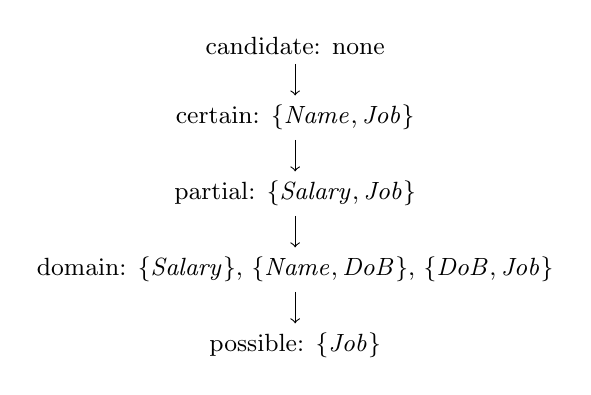
\begin{tikzpicture}[every node/.style={font=\small}, node distance=4mm and 9mm]
\node (cand) {candidate: none};
\node (cert) [below=of cand] {certain: $\{\mathit{Name},\mathit{Job}\}$};
\node (part) [below=of cert] {partial: $\{\mathit{Salary},\mathit{Job}\}$};
\node (domn) [below=of part] {domain: $\{\mathit{Salary}\}$, $\{\mathit{Name},\mathit{DoB}\}$, $\{\mathit{DoB},\mathit{Job}\}$};
\node (poss) [below=of domn] {possible: $\{\mathit{Job}\}$};
\draw[->] (cand) -- (cert); \draw[->] (cert) -- (part);
\draw[->] (part) -- (domn); \draw[->] (domn) -- (poss);
\end{tikzpicture}}
\caption{Minimal keys on $i_0$ by class (each level lists the minimal keys of that
class that are not already minimal keys of a stronger class)}
\label{fig:hierarchy}
\Description{}
\end{figure}

\subsection{Why implication matters: covers and indexes}\label{sec:why}

Suppose a schema designer, or a key-mining tool, has produced the set
\begin{align*}
\Sig_0 = \{\ &\pos{\mathit{Job}},\ \dom{\mathit{Salary}},\ \pk{\mathit{Salary},\mathit{Job}},\\
&\ck{\mathit{Name},\mathit{Job}},\ \sql{NOT NULL}(\mathit{Name})\ \}
\end{align*}
on \textsc{Staff} and asks whether $\dom{\mathit{Salary},\mathit{Job}}$ should be
added, whether $\pos{\mathit{Job}}$ is still needed, and whether
$\ck{\mathit{Salary},\mathit{Job}}$ follows. Each answer is an implication question,
and the answers decide which \sql{UNIQUE} indexes exist and which triggers fire on
every insert. Section~\ref{sec:indexing} explains how each class is enforced with the
index types that commercial systems offer; the results of
Sections~\ref{sec:axiom} and~\ref{sec:limits} say when such an index is redundant,
and how hard it is to find out. For $\Sig_0$ the answers are: yes, $\dom{\mathit{Salary},
\mathit{Job}}$ is implied (by weakening $\pk{\mathit{Salary},\mathit{Job}}$); no,
$\pos{\mathit{Job}}$ is not implied by the rest; and no, $\ck{\mathit{Salary},
\mathit{Job}}$ does not follow---the construction in the proof of
Theorem~\ref{thm:certain} produces the counterexample $\{(\text{Eve},\nul,\nul,\text{Clerk}),
(\text{Eve},\nul,80\mathrm k,\nul)\}$, in which the two records are compatible on
$\mathit{Salary}$ and $\mathit{Job}$ but neither subsumes the other.

Run on $i_0$, per-class key mining~\cite{KoehlerL25} returns ten minimal keys:
the minimal keys of each class shown in Figure~\ref{fig:hierarchy} together with
those it omits because they are also minimal in a stronger class. Their cover has
six keys. The four removed keys---$\pos{\mathit{Salary}}$,
$\pos{\mathit{Name},\mathit{DoB}}$, $\dom{\mathit{Name},\mathit{Job}}$ and
$\pk{\mathit{Name},\mathit{Job}}$---are each a weaker class on the column set of a
stronger mined key, and the 15 indexes of Section~\ref{sec:indexing} fall to 10.
On $c_0$, mining returns the three single columns as
possible and as domain keys, the three pairs of channels as partial keys, and
$\ck{\mathit{Email},\mathit{Phone},\mathit{Handle}}$. The cover again has six of
these ten keys, but it removes the certain key for a different reason: no single
key implies it, yet the three partial keys do, because their hypergraph on the
three channels is a triangle, which has no proper 2-colouring
(Theorem~\ref{thm:certain}). This saves the 8 filtered indexes of the certain
key, 15 instead of 26 indexes in all. Experiment~E finds the first pattern on the
21 tables of a real database; Experiment~C shows how often the second arises when
binary partial keys accumulate. The same shape arises on real data: on the VOC
database, three mined partial keys of \textsc{voyages} imply a four-column certain
key that none of them implies alone (Section~\ref{sec:expE}), although there a
mined certain key already implies it.

\subsection{Indexing techniques for the five classes}\label{sec:indexing}

Every class can be enforced by indexes and, where necessary, a trigger that uses them;
the hierarchy is mirrored by a hierarchy of index techniques.

\paragraph{Possible keys.} The B$^+$-tree \sql{UNIQUE} index is exactly a possible
key: the SQL standard treats null entries as distinct, so two null-bearing keys never
collide~\cite{DD97}. Oracle goes further and omits all-null entries from the
index~\cite{OracleDoc}.

\paragraph{Domain keys.} A domain key is a unique index in which nulls are
\emph{not} distinct. Several systems offer this directly: SQL Server's unique indexes
treat nulls as equal~\cite{SQLServerDoc}, PostgreSQL~15 added the clause \sql{UNIQUE
NULLS NOT DISTINCT}~\cite{PGDoc}, and Db2 offers it as an option of \sql{CREATE
UNIQUE INDEX}~\cite{Db2Doc}. Where it is absent, a unique index on the expression
$\sql{coalesce}(A,\sigma_A)$ for a sentinel $\sigma_A$ outside $\mathrm{dom}(A)$
has the same effect. So $\dom{\mathit{Country},\mathit{Product}}$ of the pricing
example costs one ordinary index.

\paragraph{Partial keys.} A partial key is enforced by one \emph{filtered} (partial)
unique index per null pattern plus a containment check. For $\pk{K}$ with nullable
columns $N_K$, create for each $P\subseteq N_K$ the index
\[
\sql{UNIQUE}(K\setminus P)\ \sql{WHERE}\ \bigwedge_{A\in P} A\ \sql{IS NULL}
\]
(SQL Server, PostgreSQL, SQLite and Db2 support filtered
indexes~\cite{SQLServerDoc,PGDoc,Db2Doc}). These indexes
reject two records with the same null pattern that agree elsewhere. A record $t$
with null pattern $P$ is subsumed by a record $t'$ with a pattern $P'\subsetneq P$
iff $t$ and $t'$ agree on $K\setminus P$; this is a point lookup of $t$'s non-null
values in the index for pattern $P'$, restricted to its leading columns. A \sql{BEFORE
INSERT} trigger issues one such lookup per $P'\subseteq P$, i.e.\ at most $2^{|P|}$
index probes, which is small because $|P|$ is the number of nulls in the new record.
In $i_0$, $\pk{\mathit{Salary},\mathit{Job}}$ needs the four indexes for
$P\in\{\emptyset,\{\mathit{Salary}\},\{\mathit{Job}\},\{\mathit{Salary},
\mathit{Job}\}\}$, and inserting $(\text{Ann},\nul,90\mathrm k,\nul)$ probes the
indexes for $\emptyset$ and $\{\mathit{Job}\}$ with the value $90\mathrm k$, finds
record 2, and rejects the insert.

\paragraph{Certain keys.} A certain key forbids \emph{compatible} records, which need
not have nested null patterns, so index probes must look in both directions. With the
same family of filtered indexes, a new record $t$ with non-null columns
$K\setminus P$ is compatible with an existing $t'$ iff for every $A\in K\setminus P$,
$t'(A)=t(A)$ or $t'(A)=\nul$. For each $P'\subseteq N_K$ the trigger probes the
index for $P'$ with the values of $t$ on $(K\setminus P)\setminus P'$, giving
$2^{|N_K|}$ probes in the worst case. K\"ohler et al.~\cite{KLLZ16} show that for
certain keys with few nullable columns this is competitive with a single
\sql{UNIQUE} index; rule R4 of Section~\ref{sec:rules} explains why: with one
nullable column a certain key \emph{is} a partial key and needs only two indexes.

\paragraph{Candidate keys.} A candidate key is a \sql{UNIQUE} index on \sql{NOT
NULL} columns, the base case in which all five techniques coincide, as the five
classes do on \sql{NOT NULL} columns (rule R3).

\paragraph{An emulation.} These techniques use only features that major systems
already offer, to emulate what a system with native partial and certain keys would
do internally. The value of a cover does not depend on them: any enforcement whose
cost grows with the number of declared keys gains from enforcing fewer.

\paragraph{What implication buys.} Each redundant key saves its indexes and probes.
The number of indexes for a partial or certain key grows as $2^{|N_K|}$, so detecting
that $\ck{K}$ is implied---for instance by a triangle of binary partial keys that
are already enforced for their own reasons---saves the most expensive structures. The
results below show that this detection is trivial for four classes and, for certain
keys, equivalent to hypergraph 2-colourability.

\subsection{Beyond enforcement: query optimisation}\label{sec:qopt}

Each class makes one notion of matching unique, and each notion is the semantics of
a family of SQL constructs (Table~\ref{tab:qopt}); a key of the class lets an
optimiser prove ``at most one match'' for those constructs, e.g.\ that a
\sql{DISTINCT} over columns containing $K$ is a no-op under $\dom K$, though not under
\sql{UNIQUE}, that a partial key makes the minimum-union step of outer-join
reordering~\cite{GL94} a no-op, and that key rewrites under a certain key stay sound
under certain-answer semantics~\cite{GL16}. The class a construct needs may be implied rather than declared, so an
optimiser should reason from the cover with the implication test of
Section~\ref{sec:algorithms}; Experiment~F (Section~\ref{sec:expF}) measures these
rewrites on real tables.

\begin{table}[t]
\centering
\caption{The notion of match each class makes unique, the SQL constructs with that
semantics, and the rewrites a key of the class licenses}
\label{tab:qopt}
\small
\adjustbox{max width=\columnwidth}{\begin{tabular}{l p{2.6cm} p{3.2cm} p{3.6cm}}
\toprule
Class & Rows match on $K$ if & SQL constructs & Licensed rewrite \\
\midrule
possible & equal, non-null & \sql{=}, equi-joins, \sql{IN} & unique lookup and join partner; join elimination \\
domain & equal, \nul\ $=$ \nul & \sql{GROUP BY}, \sql{DISTINCT}, set operations, \sql{IS NOT DISTINCT FROM} & drop \sql{DISTINCT}; \sql{GROUP BY} $K$ as projection \\
partial & one subsumes the other & outer joins, full disjunction, record merging & drop subsumption removal \\
certain & compatible & wildcard matching, certain answers & one compatible match per total probe; rewrites sound in every completion \\
\bottomrule
\end{tabular}}
\end{table}


\section{An Axiomatisation of Implication}\label{sec:axiom}

Readers interested only in computing covers need Theorem~\ref{thm:certain} of
this section, Section~\ref{sec:covers} and Algorithms~\ref{alg:decide}--\ref{alg:cover-general};
the rest of this section and Section~\ref{sec:limits} establish completeness and
limits.

\paragraph{Two-tuple witnesses.}\label{sec:pairs} Every class constrains pairs of
tuples only, so $\Sig\not\models\varphi$ iff some two-tuple instance satisfies
$\Sig$ and violates $\varphi$ (Appendix~\ref{app:pairs}). Such an instance is
described by a type per column: \bn\ (both null), \eq\ (equal non-null values),
\nv\ or \vn\ (exactly one null), \dd\ (distinct non-null values), with only \eq\ and
\dd\ on \sql{NOT NULL} columns. A pair satisfies $\ck L$ iff some column of $L$ is
\dd; $\pk L$ iff $L$ has a column of type \vn\ or \dd\ and one of type \nv\ or \dd;
$\dom L$ iff some column of $L$ is not \bn\ or \eq; $\pos L$ iff some column of $L$
is not \eq\ (Lemma~\ref{lem:typing}). No key is valid, so a sound inference system
has no axioms.

\subsection{Inference Rules and Soundness}\label{sec:rules}
%=====================================================================

Let $\mathcal R$ consist of the rules in Table~\ref{tab:rules}, where $X,K,L$ range
over column sets, $A,B,C$ over columns, and side conditions refer to the schema's
$\NN$.

\begin{table}[t]
\centering
\caption{The inference rules}
\label{tab:rules}
\adjustbox{max width=\columnwidth}{\begin{tabular}{l l l l}
\toprule
Rule & Premises & Conclusion & Side condition \\
\midrule
R1 (weakening) & $\ck{K}$ & $\pk{K}$ & \\
 & $\pk{K}$ & $\dom{K}$ & \\
 & $\dom{K}$ & $\pos{K}$ & \\
 & $\cand{K}$ & $\ck{K}$ & \\
 & $\ck{K}$ & $\cand{K}$ & $K\subseteq\NN$ \\
R2 (superkey) & $\mathcal C(K)$ & $\mathcal C(KL)$ & $KL\subseteq\NN$ if $\mathcal C$ is candidate \\
R3 (total collapse) & $\pos{K}$ & $\ck{K}$ & $K\subseteq\NN$ \\
R4 (one-nullable collapse) & $\pk{XA}$ & $\ck{XA}$ & $X\subseteq\NN$ \\
R5 (triangle) & $\pk{XAB},\pk{XAC},\pk{XBC}$ & $\ck{XABC}$ & $X\subseteq\NN$ \\
\bottomrule
\end{tabular}}
\end{table}

R1 and R2 are the rules of a single class lifted along the hierarchy. R3 is the rule
of~\cite{KLLZ16} that all classes coincide on total columns, extended to five
classes. R4 and R5 are the new interaction rules between partial and certain keys.
R4 says that subsumption-freedom and compatibility-freedom coincide when at most one
key column may carry nulls; it explains why almost every meaningful partial key mined from the Hockey tables
in~\cite{KoehlerL25} is also certain (27 of 29), as few of them have two nullable
columns. R5 is a pigeonhole rule; Section~\ref{sec:certain} shows it is the
smallest member of an infinite family.

\begin{theorem}[Soundness]\label{thm:sound}
Every rule of $\mathcal R$ is sound.
\end{theorem}
\noindent\emph{Proof idea.} By Lemmas~\ref{lem:pair} and~\ref{lem:typing} it suffices to check each rule on a typed two-tuple instance: the type sets of the classes are nested (R1), the conditions are monotone under enlarging the key (R2), and they collapse on \sql{NOT NULL} columns (R3) and on a single nullable column (R4). Full proof in Appendix~\ref{app:proofs}.

\begin{example}[R5 on \textsc{Contact}]\label{ex:triangle}
Declare $\pk{\mathit{Email},\mathit{Phone}}$, $\pk{\mathit{Email},\mathit{Handle}}$
and $\pk{\mathit{Phone},\mathit{Handle}}$: nobody is stored once with two channels
and once with only one of them. R5 derives $\ck{\mathit{Email},\mathit{Phone},
\mathit{Handle}}$: any two records differ on a channel both have. Concretely, a
second record compatible with $(\mathtt{a@x.org},\ \nul,\ \mathtt{@ann})$ on all
three columns must have a value or null on each; if it has $\mathtt{a@x.org}$ it is
subsumed or subsuming on $\{\mathit{Email},\mathit{Handle}\}$ unless its handle is
\emph{different} and non-null, which breaks compatibility. Working through the
cases is exactly the pigeonhole argument. The three binary partial keys thus make the
$2^3=8$ filtered indexes of Section~\ref{sec:indexing} for the certain key
redundant. All four keys hold on the instance $c_0$ of
Section~\ref{sec:motivation}: no row is subsumed by another on any pair of
channels, and any two rows differ on a channel both have.
\end{example}

By contrast, Example~3 of~\cite{KoehlerL25}---$\pk{\mathit{playerID},\mathit{coachID},
\mathit{hofID}}$ on the Hockey table \textsc{Master}, which is not a certain
key---is a single partial key with three nullable columns, and no rule of
$\mathcal R$ upgrades it. Section~\ref{sec:certain} shows that nothing should: a
single 3-edge is 2-colourable.


\subsection{Completeness for possible, domain, partial and candidate targets}\label{sec:completeness}
%=====================================================================

Write $\Sig^+$ for the closure of $\Sig$ under R1--R4.

\begin{theorem}\label{thm:complete}
Let $\varphi$ be $\pos{K}$, $\dom{K}$, $\pk{K}$ or $\cand{K}$. If
$\varphi\notin\Sig^+$ then $\Sig\not\models\varphi$.
\end{theorem}
\noindent\emph{Proof idea.} For a target that is not derivable we build a type assignment, hence a two-tuple instance, that violates the target and satisfies every premise: columns outside $K$ get type \dd, \sql{NOT NULL} columns of $K$ get \eq, and the nullable columns of $K$ get the one type that breaks the target class but no premise inside $K$. Full proof in Appendix~\ref{app:proofs}.



\begin{corollary}\label{cor:fragments}
Every set of classes not containing both partial and certain keys is finitely
axiomatised by those rules among R1--R4 that mention only its classes. In
particular possible and certain keys with \sql{NOT NULL} are axiomatised by R1, R2,
R3, recovering~\cite{KLLZ16}.
\end{corollary}
\noindent\emph{Proof idea.} Without partial premises condition (iii) of Theorem~\ref{thm:certain} is void, and (i), (ii) are derivable by R1--R3. Full proof in Appendix~\ref{app:proofs}.


\subsection{Certain Keys and Hypergraph 2-Colourability}\label{sec:certain}
%=====================================================================

For a certain target, implication from partial keys is a 2-colouring problem. Fix
$K\subseteq S$ and let $N_K:=K\cap N$ be its nullable columns. Define the hypergraph
\[
H(\Sig,K) := \bigl(N_K,\ \{\,L\cap N_K : \pk{L}\in\Sig,\ L\subseteq K\,\}\bigr).
\]
A 2-colouring $c:N_K\to\{\text{red},\text{blue}\}$ is \emph{proper} if every edge
contains a vertex of each colour. An edge of size at most one, in particular the
empty edge contributed by a partial key $L\subseteq K\cap\NN$, admits no proper
colouring.

\begin{theorem}\label{thm:certain}
$\Sig\models\ck{K}$ iff at least one of the following holds:
\begin{enumerate}
\item[(i)] $\ck{L}\in\Sig$ or $\cand{L}\in\Sig$ for some $L\subseteq K$;
\item[(ii)] $\pos{L}\in\Sig$ or $\dom{L}\in\Sig$ for some $L\subseteq K\cap\NN$;
\item[(iii)] $H(\Sig,K)$ has no proper 2-colouring.
\end{enumerate}
\end{theorem}
\noindent\emph{Proof idea.} A two-tuple instance violating $\ck K$ gives every nullable column of $K$ the type \vn\ or \nv, a 2-colouring; a partial premise $\pk L$ with $L\subseteq K$ is satisfied iff $L$ sees both colours. So counter-instances are exactly the proper 2-colourings of $H(\Sig,K)$. Full proof in Appendix~\ref{app:proofs}.

\begin{example}
\emph{(a)} For $\Sig_0$ of Section~\ref{sec:why} and $K=\{\mathit{Salary},
\mathit{Job}\}$: (i) fails, (ii) fails, and $H(\Sig_0,K)$ has the single edge
$\{\mathit{Salary},\mathit{Job}\}$, properly coloured by $\mathit{Salary}\mapsto$
red, $\mathit{Job}\mapsto$ blue. The construction gives $\tau(\mathit{Salary})=\vn$,
$\tau(\mathit{Job})=\nv$, $\tau(\mathit{Name})=\tau(\mathit{DoB})=\dd$, i.e.\ the
counterexample announced in Section~\ref{sec:why}.
\emph{(b)} In Example~\ref{ex:triangle}, $H$ is the triangle on $\{\mathit{Email},
\mathit{Phone},\mathit{Handle}\}$, which is not 2-colourable, so the certain key is
implied.
\emph{(c)} On the Hockey table \textsc{Master}, $\Sig=\{\pk{\mathit{playerID},
\mathit{coachID},\mathit{hofID}}\}$ gives a hypergraph with one edge of size three,
2-colourable by colouring one vertex red and two blue; the certain key is not
implied, in agreement with Example~3 of~\cite{KoehlerL25}.
\end{example}

The rules of Section~\ref{sec:rules} are the smallest cases of (iii): R3 and R4 are
the edges of size zero and one, R5 the 3-cycle. Theorem~\ref{thm:certain} also shows what is
missing: every non-2-colourable hypergraph without a triangle, such as a 5-cycle,
yields an implication that R1--R5 cannot derive; adding one rule per such
hypergraph gives a complete infinite system
(Corollary~\ref{cor:infinite}, Appendix~\ref{app:examples}).



\section{Limits of Implication}\label{sec:limits}\label{sec:nonfinite}\label{sec:complexity}\label{sec:maximal}

The combined class has no sound and complete inference system with a bound on the
number of premises per rule. The witnesses are odd cycles of binary partial keys:
for $k\ge1$ let $S_k:=\{A_1,\dots,A_{2k+1}\}$, $\NN:=\emptyset$ and
$\Sig_k:=\{\pk{A_iA_{i+1}}\}$ with indices modulo $2k+1$. Read $\Sig_2$ as five
pairwise dirty-data checks on five alternative identifiers of a person: it implies
$\ck{A_1\cdots A_5}$, any two records differ on an identifier both possess, but
no proper subset of the checks implies any certain key
(Lemma~\ref{lem:cycle}, Appendix~\ref{app:examples}).

\begin{theorem}\label{thm:nonfinite}
For no $m$ is there a sound and complete inference system for the combined class of
keys in which every rule has at most $m$ premises. The same holds for the class of
partial and certain keys alone over schemas without \sql{NOT NULL} constraints. In
particular, neither class is finitely axiomatisable.
\end{theorem}
\noindent\emph{Proof idea.} With premise bound $m$ take the odd cycle with $2k+1>m$ edges: the first certain conclusion in any derivation rests on at most $m$ premises, which by Lemma~\ref{lem:cycle}(b) do not imply it. Full proof in Appendix~\ref{app:proofs}.

The failure is not the unbounded-chain phenomenon of functional dependencies:
every key implied by a proper sub-cycle is a mere superkey of a premise, so no
useful intermediate key exists. It is also sharp, as the fragments below show.

\begin{theorem}\label{thm:conp}
Deciding $\Sig\models\varphi$ for the combined class of keys with \sql{NOT NULL}
constraints is coNP-complete.
\end{theorem}
\noindent\emph{Proof idea.} Membership: a counter-instance is a type assignment, checked in linear time. Hardness: from 2-colourability of 3-uniform hypergraphs, with one ternary partial key per edge and the certain key on all vertices as target. Full proof in Appendix~\ref{app:proofs}.

Table~\ref{tab:complexity} summarises the tractable cases: only partial keys
with three or more nullable columns interacting with a certain target are hard.
For the first three rows a cover is computable in polynomial time; in the last row
each test is coNP-complete, but the hypergraph has as many vertices as the target
has nullable columns, typically a handful, and a declared certain key whose
hypergraph is non-2-colourable is enforced for free by the filtered indexes of its
partial keys---the most valuable redundancy to detect, since its own index family
is the largest.

\begin{table}[t]
\centering
\caption{Complexity of implication by fragment}
\label{tab:complexity}
\adjustbox{max width=\columnwidth}{\begin{tabular}{p{2.9cm} p{1.5cm} p{3.1cm}}
\toprule
Fragment & Complexity & Reason \\
\midrule
Target possible, domain, partial or candidate & polynomial & closure under R1--R4 (Theorem~\ref{thm:complete}) \\
No partial keys in $\Sig$ & polynomial & conditions (i), (ii) only \\
Every partial key in $\Sig$ has at most two nullable columns & polynomial & $H(\Sig,K)$ is a graph; 2-colourability is bipartiteness \\
Partial keys with three nullable columns, certain target & coNP-complete & Theorem~\ref{thm:conp} \\
\bottomrule
\end{tabular}}
\end{table}

For a set $\mathcal F$ of class names, the \emph{$\mathcal F$-fragment} is the
implication problem with premises and target in $\mathcal F$, over schemas with
arbitrary \sql{NOT NULL} constraints.

\begin{theorem}\label{thm:maximal-classes}
The $\mathcal F$-fragment is finitely axiomatisable iff $\mathcal F$ does not contain
both partial and certain keys. Consequently the maximal finitely axiomatisable
fragments are exactly
\begin{align*}
\mathcal F_1&=\{\text{possible},\text{domain},\text{partial},\text{candidate}\}\quad\text{and}\\
\mathcal F_2&=\{\text{possible},\text{domain},\text{certain},\text{candidate}\}.
\end{align*}
$\mathcal F_1$ is axiomatised by R1, R2 and the instance $\pos{K}\vdash\cand{K}$
for $K\subseteq\NN$ of R3; $\mathcal F_2$ by R1, R2 and R3.
\end{theorem}
\noindent\emph{Proof idea.} With both partial and certain keys Theorem~\ref{thm:nonfinite} applies. Without one of them condition (iii) of Theorem~\ref{thm:certain} is void or trivial, and R1--R4 are complete. Full proof in Appendix~\ref{app:proofs}.

$\mathcal F_2$ is the system of~\cite{KLLZ16} extended by domain keys, which
therefore come for free; $\mathcal F_1$ shows that partial keys are equally harmless
as long as certain keys are not targets.

\section{Minimal and Optimal Covers Are Unique}\label{sec:covers}
%=====================================================================

A \emph{cover} of $\Sig$ is a set $\Gamma$ of keys with $\Gamma\models\Sig$ and
$\Sig\models\Gamma$. A cover is \emph{minimal} if no cover has fewer keys and
\emph{optimal} if no cover has fewer \emph{attribute occurrences}
$\|\Gamma\|=\sum_{\mathcal C(K)\in\Gamma}|K|$. Covers are what a system actually
enforces: each key of the cover is an index family and a trigger
(Section~\ref{sec:indexing}), so a minimal cover minimises the number of enforced
constraints and an optimal cover minimises the total index width. For functional
dependencies the two notions differ and optimal covers are hard to find; for the
key classes studied here they coincide, and the cover is unique.

Two keys are \emph{equivalent}, $\varphi\equiv\psi$, if each implies the other.
By R1, R3 and R4 and Lemma~\ref{lem:cand}, $\mathcal C(K)\equiv\mathcal C'(K')$ iff
$K=K'$ and one of: $\mathcal C=\mathcal C'$; $K\subseteq\NN$ (all classes coincide);
or $\{\mathcal C,\mathcal C'\}=\{\text{partial},\text{certain}\}$ and
$|K\setminus\NN|\le1$ (R4). A set $\Sig$ is \emph{non-redundant} if
$\Sig\setminus\{\sigma\}\not\models\sigma$ for every $\sigma\in\Sig$; in particular
it contains no two equivalent keys.

\subsection{Deciding implication}\label{sec:algorithms}
%=====================================================================

Theorems~\ref{thm:complete} and~\ref{thm:certain} turn directly into a decision
procedure for the whole class. It is polynomial in the sizes of $\Sig$ and $S$ and
exponential only in the number of partial keys with three or more nullable columns
inside the target key, which is also where the coNP lower bound of
Theorem~\ref{thm:conp} lives. Throughout, $\|\Sig\|:=\sum_{\mathcal C(L)\in\Sig}|L|$,
$n:=|S|$, and keys are bit vectors, so a subset test costs $O(n)$.


Algorithm~\ref{alg:decide} normalises candidate keys into \sql{NOT NULL} plus
certain keys (Lemma~\ref{lem:cand}), answers the four easy target classes by one
scan of $\Sig$ (Theorem~\ref{thm:complete}), and reduces a certain target to
conditions (i)--(iii) of Theorem~\ref{thm:certain}, delegating (iii) to
Algorithm~\ref{alg:colour}. We write $\mathcal C'\succeq\mathcal C$ when $\mathcal C'$
is at least as strong as $\mathcal C$ in the order candidate $\succ$ certain $\succ$
partial $\succ$ domain $\succ$ possible.

\begin{algorithm}[t]
\caption{\textsc{Implies}$((S,\NN),\Sig,\mathcal C(K))$ --- decides $\Sig\models\mathcal C(K)$}
\label{alg:decide}
\begin{algorithmic}[1]
\State \textbf{for each} $\cand{L}\in\Sig$: $\NN\gets\NN\cup L$ and replace $\cand{L}$ by $\ck{L}$
\If{$\mathcal C=$ candidate} \Comment{Lemma~\ref{lem:cand}}
  \State \textbf{if} $K\not\subseteq\NN$ \textbf{then return} \textsc{false}
  \State $\mathcal C\gets$ certain
\EndIf
\If{$\mathcal C\in\{$possible, domain, partial$\}$} \Comment{Theorem~\ref{thm:complete}}
  \ForAll{$\mathcal C'(L)\in\Sig$ with $L\subseteq K$}
    \State \textbf{if} $\mathcal C'\succeq\mathcal C$ \textbf{or} $L\subseteq\NN$ \textbf{then return} \textsc{true}
  \EndFor
  \State \Return \textsc{false}
\EndIf
\State $E\gets\emptyset$; $N_K\gets K\setminus\NN$ \Comment{target is $\ck{K}$; Theorem~\ref{thm:certain}}
\ForAll{$\mathcal C'(L)\in\Sig$ with $L\subseteq K$}
  \State \textbf{if} $\mathcal C'=$ certain \textbf{or} $L\subseteq\NN$ \textbf{then return} \textsc{true} \Comment{(i), (ii)}
  \State \textbf{if} $\mathcal C'=$ partial \textbf{then} $E\gets E\cup\{L\cap N_K\}$
\EndFor
\State \Return \textsc{NotTwoColourable}$(N_K,E)$ \Comment{(iii)}
\end{algorithmic}
\end{algorithm}


Algorithm~\ref{alg:colour} decides
whether a hypergraph $(V,E)$ has no proper 2-colouring. It returns true at once if
some edge has at most one vertex, keeps only minimal edges, and splits $E$ into the
binary edges $E_2$ and the larger edges $e_1,\dots,e_h$. It then branches: for each
$e_j$ it fixes a vertex $v\in e_j$ and tries, for every $w\in e_j\setminus\{v\}$,
adding the binary edge $\{v,w\}$ (some $w$ must receive the colour opposite to
$v$); a leaf of the branching holds a graph $F\supseteq E_2$ on $V$, and the
hypergraph is non-2-colourable iff every leaf's $F$ is non-bipartite, which a
linear-time breadth-first search decides.

\begin{algorithm}[t]
\caption{\textsc{NotTwoColourable}$(V,E)$ --- decides whether $(V,E)$ has no proper
2-colouring}
\label{alg:colour}
\begin{algorithmic}[1]
\State \textbf{if} some $e\in E$ has $|e|\le1$ \textbf{then return} \textsc{true}
\State remove from $E$ every edge that strictly contains another edge
  \Comment{minimal edges suffice}
\State remove from $V$ every vertex lying in no edge
\State $E_2\gets\{e\in E:|e|=2\}$;\quad $E_3\gets\{e\in E:|e|\ge3\}=\{e_1,\dots,e_h\}$
\State \Return \textsc{Branch}$(1,E_2)$
\Statex
\Procedure{Branch}{$j,F$} \Comment{$F$: a graph on $V$; $e_1,\dots,e_{j-1}$ already split}
  \State \textbf{if} $j>h$ \textbf{then return not} \textsc{Bipartite}$(V,F)$
  \State let $v$ be a fixed vertex of $e_j$
  \ForAll{$w\in e_j\setminus\{v\}$} \Comment{some $w$ gets the colour opposite to $v$}
    \State \textbf{if not} \textsc{Branch}$(j+1,F\cup\{\{v,w\}\})$ \textbf{then return} \textsc{false}
  \EndFor
  \State \Return \textsc{true}
\EndProcedure
\end{algorithmic}
\end{algorithm}


\begin{theorem}[Correctness]\label{thm:algcorrect}
Algorithm~\ref{alg:decide} returns \textsc{true} iff $\Sig\models\mathcal C(K)$.
\end{theorem}
\noindent\emph{Proof idea.} Lines~1--11 implement R1--R4, complete by Theorem~\ref{thm:complete}; lines~12--17 implement condition (iii) of Theorem~\ref{thm:certain} through Algorithm~\ref{alg:colour}. Full proof in Appendix~\ref{app:proofs}.


\begin{theorem}[Running time and space]\label{thm:algcost}
Let $N_K$ be the nullable columns of the target, $E$ the minimal edge set of
$H(\Sig,K)$ after lines~1--3 of Algorithm~\ref{alg:colour}, $m:=|E|$, and
$e_1,\dots,e_h$ its edges of size at least three. Algorithm~\ref{alg:decide} runs in
time
\[
O\bigl(\,|\Sig|\cdot n\ +\ m^2 n\ +\ \textstyle\prod_{j=1}^{h}(|e_j|-1)\cdot(|N_K|+m)\,\bigr)
\]
and $O(|\Sig|\cdot n+m\,n+h)$ bits of space. It is linear for a possible,
domain, partial or candidate target, polynomial for a certain target when every
partial key has at most two nullable columns ($h=0$), and fixed-parameter
tractable in $|N_K|$ in general, the exponential factor being at most
$2^{|N_K|-1}$.
\end{theorem}
\noindent\emph{Proof idea.} One subset test per premise; for a certain target, one branch per choice of a pair from each edge of three or more vertices, each followed by a linear bipartiteness test. Full proof in Appendix~\ref{app:proofs}.



\paragraph{Computing a non-redundant cover.} Removing every implied key from $\Sig$
costs $|\Sig|$ calls of Algorithm~\ref{alg:decide} on $\Sig\setminus\{\varphi\}$, so a
cover free of implied keys, and with it a minimal family of unique and filtered
indexes (Section~\ref{sec:indexing}), is computed in time $O(|\Sig|^2 n)$ plus the
colouring term for each certain key in $\Sig$. In practice the colouring term is
negligible, since $|N_K|$ is the number of nullable columns of one key.


\subsection{The maximal fragments}

In $\mathcal F_1$ and $\mathcal F_2$ implication is \emph{single-premise}. Write
$\mathcal C_1\prec\mathcal C_2\prec\mathcal C_3$ for the three non-candidate
classes of the fragment in increasing strength (possible $\prec$ domain $\prec$
partial in $\mathcal F_1$, possible $\prec$ domain $\prec$ certain in
$\mathcal F_2$). By Theorem~\ref{thm:complete}, and Theorem~\ref{thm:certain} with
$E=\emptyset$ for $\mathcal F_2$,
\begin{equation}\label{eq:impl-frag}
\begin{split}\Sig\models\mathcal C(K)\iff{}&\text{some }\mathcal C'(L)\in\Sig\text{ has }L\subseteq K\\
&\text{and }(\mathcal C'\succeq\mathcal C\ \text{or}\ L\subseteq\NN),\end{split}
\end{equation}
where candidate counts as the strongest class and, by Lemma~\ref{lem:cand}, occurs
only on total sets. Hence $\Sig\models\varphi$ iff $\{\sigma\}\models\varphi$ for
some $\sigma\in\Sig$, and this alone determines the covers.

\begin{theorem}\label{thm:cover-frag}
Let $\Sig$ be a non-redundant set of keys of $\mathcal F_1$ or $\mathcal F_2$. Every
cover $\Gamma$ of $\Sig$ contains, for each $\sigma\in\Sig$, a key equivalent to
$\sigma$. Consequently, for every set $\Sig_0$ of keys of the fragment, any
non-redundant cover of $\Sig_0$ is, up to equivalence, the unique minimal cover and
the unique optimal cover of $\Sig_0$.
\end{theorem}
\begin{proof}
Let $\sigma\in\Sig$. Since $\Gamma\models\sigma$ and implication is single-premise,
some $\gamma\in\Gamma$ satisfies $\gamma\models\sigma$. Since $\Sig\models\gamma$,
some $\sigma'\in\Sig$ satisfies $\sigma'\models\gamma$, hence
$\sigma'\models\sigma$. As $\Sig$ is non-redundant, $\sigma'=\sigma$, so
$\sigma\models\gamma\models\sigma$ and $\gamma\equiv\sigma$. Distinct keys of $\Sig$
are inequivalent (non-redundancy), so distinct $\sigma$ yield distinct $\gamma$;
thus $|\Gamma|\ge|\Sig|$, and since equivalent keys have the same column set,
$\|\Gamma\|\ge\|\Sig\|$. For the consequence, let $\Gamma_1,\Gamma_2$ be
non-redundant covers of $\Sig_0$. Both are covers of each other, so each contains
an equivalent of every key of the other, i.e.\ they coincide up to equivalence;
and any cover $\Gamma$ of $\Sig_0$ is a cover of $\Gamma_1$, whence
$|\Gamma|\ge|\Gamma_1|$ and $\|\Gamma\|\ge\|\Gamma_1\|$.
\end{proof}

No cover can therefore profit from keys outside $\Sig_0$, and minimising the
number of keys and the number of attribute occurrences are achieved by the same
set. Algorithm~\ref{alg:cover-frag} computes it in one pass.

\begin{algorithm}[t]
\caption{\textsc{MinCover}$_{\mathcal F}((S,\NN),\Sig)$ --- the unique minimal and
optimal cover in $\mathcal F_1$ or $\mathcal F_2$}
\label{alg:cover-frag}
\begin{algorithmic}[1]
\State \textbf{for each} $\cand{L}\in\Sig$: $\NN\gets\NN\cup L$; replace $\cand{L}$ by $\mathcal C_3(L)$
\State \textbf{for each} $\mathcal C(L)\in\Sig$ with $L\subseteq\NN$: replace $\mathcal C$ by $\mathcal C_3$
\State remove duplicate keys
\State sort $\Sig$ by $|L|$ ascending, ties by class descending ($\mathcal C_3$ first)
\State $\Gamma\gets\emptyset$
\ForAll{$\sigma=\mathcal C(K)$ in sorted order}
  \State $\mathit{red}\gets\textsc{false}$
  \ForAll{$\gamma=\mathcal C'(L)\in\Gamma$}
    \If{$L\subseteq K$ \textbf{and} ($\mathcal C'\succeq\mathcal C$ \textbf{or} $L\subseteq\NN$)}
      \State $\mathit{red}\gets\textsc{true}$; \textbf{break}
    \EndIf
  \EndFor
  \State \textbf{if not} $\mathit{red}$ \textbf{then} $\Gamma\gets\Gamma\cup\{\sigma\}$
\EndFor
\State \Return $\Gamma$
\end{algorithmic}
\end{algorithm}

\begin{theorem}\label{thm:cover-frag-alg}
Algorithm~\ref{alg:cover-frag} returns a non-redundant cover of $\Sig$, hence by
Theorem~\ref{thm:cover-frag} the unique minimal and optimal cover up to
equivalence. It runs in time $O(|\Sig|^2\,n)$ and space $O(|\Sig|\,n)$ bits.
\end{theorem}
\noindent\emph{Proof idea.} Keys are processed by size, then strength, so a key is redundant iff a kept key is contained in it with at least its strength, by~\eqref{eq:impl-frag}. Full proof in Appendix~\ref{app:proofs}.

\subsection{The general class}

When partial and certain keys coexist, implication of a certain key is no longer
single-premise (Section~\ref{sec:certain}), so one might hope to shrink a cover by
trading a wide certain key for narrower partial keys. This never helps: the
non-redundant subset remains the unique minimal and optimal cover. What changes is
only the cost of the redundancy test.

\begin{theorem}\label{thm:cover-general}
Let $\Sig$ be a non-redundant set of keys of the combined class. Every cover
$\Gamma$ of $\Sig$ contains, for each $\sigma\in\Sig$, a key equivalent to
$\sigma$. Consequently any non-redundant cover of any set $\Sig_0$ is, up to
equivalence, the unique minimal and the unique optimal cover of $\Sig_0$.
\end{theorem}
\noindent\emph{Proof idea.} Fix $\sigma\in\Sig$. Since $\Gamma\models\sigma$, some key of $\Gamma$ implies $\sigma$, or, for a certain $\sigma$, a set of partial keys of $\Gamma$ whose hypergraph inside $\sigma$ is not 2-colourable. Each of these is in turn implied by $\Sig$, and following the implication back into $\Sig$, non-redundancy forces the premise to be $\sigma$ itself; a non-2-colourable hypergraph cannot arise this way except as a single edge with at most one vertex, where partial and certain keys coincide (R4). So $\Gamma$ contains a key equivalent to $\sigma$, and the counting argument of Theorem~\ref{thm:cover-frag} applies. Full proof in Appendix~\ref{app:proofs}.

\begin{algorithm}[t]
\caption{\textsc{MinCover}$((S,\NN),\Sig)$ --- the unique minimal and optimal
cover in the combined class}
\label{alg:cover-general}
\begin{algorithmic}[1]
\State \textbf{for each} $\cand{L}\in\Sig$: $\NN\gets\NN\cup L$; replace $\cand{L}$ by $\ck L$
\State \textbf{for each} $\mathcal C(L)\in\Sig$ with $L\subseteq\NN$: replace $\mathcal C$ by certain
\State \textbf{for each} $\pk L\in\Sig$ with $|L\setminus\NN|\le1$: replace by $\ck L$ \Comment{R4}
\State remove duplicate keys
\State $\Gamma\gets\Sig$; sort $\Gamma$ by $|L|$ descending \Comment{wide keys are tested first}
\ForAll{$\sigma=\mathcal C(K)\in\Gamma$ in that order}
  \If{$\mathcal C\neq$ certain}
    \State $\mathit{red}\gets$ [some $\mathcal C'(L)\in\Gamma\setminus\{\sigma\}$ has $L\subseteq K$
    \Statex \hspace{\algorithmicindent}\hspace{\algorithmicindent}\hspace{\algorithmicindent} and ($\mathcal C'\succeq\mathcal C$ or $L\subseteq\NN$)]
  \Else
    \State $\mathit{red}\gets\textsc{Implies}((S,\NN),\Gamma\setminus\{\sigma\},\ck K)$ \Comment{Algorithm~\ref{alg:decide}}
  \EndIf
  \State \textbf{if} $\mathit{red}$ \textbf{then} $\Gamma\gets\Gamma\setminus\{\sigma\}$
\EndFor
\State \Return $\Gamma$
\end{algorithmic}
\end{algorithm}

\begin{theorem}\label{thm:cover-general-alg}
Algorithm~\ref{alg:cover-general} returns a non-redundant cover of $\Sig$, hence by
Theorem~\ref{thm:cover-general} the unique minimal and optimal cover up to
equivalence. Let $c$ be the number of certain keys in $\Sig$, let $m\le|\Sig|$
bound the number of partial keys inside any one certain key, and let $b$ bound the
number of nullable columns of a certain key in $\Sig$. The algorithm runs in time
\[
O\bigl(|\Sig|^2\,n\ +\ c\,(m^2n+2^{\,b-1}(b+m))\bigr)
\]
and $O(|\Sig|\,n+m\,n+b)$ bits of space. It is polynomial when every partial key
has at most two nullable columns, or when $b$ is bounded; in general each
redundancy test of a certain key is a coNP-complete problem
(Theorem~\ref{thm:conp}).
\end{theorem}
\noindent\emph{Proof idea.} A key is removed only when the remaining set implies it, so equivalence is preserved; removal shrinks the implied set, so a kept key stays non-redundant. Full proof in Appendix~\ref{app:proofs}.

\begin{example}
{\sloppy Let $\Sig$ consist of $\pk{AB}$, $\pk{AC}$, $\pk{BC}$, $\ck{ABC}$ and
$\ck{ABCD}$ over nullable $A,B,C,D$. Line~5 orders $\ck{ABCD}$ first;
Algorithm~\ref{alg:decide} finds the certain premise $\ck{ABC}$ inside $ABCD$ and
the key is removed. Next $\ck{ABC}$: there is no certain premise inside it,
$\NN=\emptyset$, and the hypergraph of the three binary partial keys is the
triangle, which is not 2-colourable; the key is removed. Each binary partial key
is then tested by the scan of line~8 against the other two and kept. The cover is
the triangle of partial keys: three keys and six attribute occurrences instead of
five keys and thirteen occurrences; in terms of Section~\ref{sec:indexing}, the
$2^3+2^4$ filtered indexes of the two certain keys are replaced by $3\cdot2^2$.
\par}
\end{example}

Theorems~\ref{thm:cover-frag} and~\ref{thm:cover-general} say that for keys with
nulls there is no design space of covers at all: the set of constraints a system
should enforce is canonical. In the maximal fragments it is computed in quadratic
time; in the combined class the only extra cost is a colouring test per certain
key, exponential only in the number of its nullable columns.


\section{Experiments}\label{sec:experiments}
%=====================================================================

We implemented the algorithms of Sections~\ref{sec:algorithms}
and~\ref{sec:covers} and ran five experiments: three on random key sets
(cover size, attribute occurrences and running time under growing input size,
growing schema size, and growing interaction between partial and certain keys),
one that enforces the input and its cover in a database and measures the cost
of inserts, updates and integrity checks, and one on the keys mined from a real
database. All code, the complete logs of every
generated input with its cover, and the raw measurements accompany the paper;
Appendix~\ref{app:repro} describes them.

\subsection{Setup}

\paragraph{Implementation.} Column sets are bit vectors; Algorithms~\ref{alg:decide},
\ref{alg:colour}, \ref{alg:cover-frag} and~\ref{alg:cover-general} are implemented
in Python~3.12 exactly as printed (\texttt{keys.py}, about 150 lines). It was validated on the examples of the paper and on 600 random instances over
3--7 columns, whose covers were checked equivalent to the input and non-redundant
by independent implication tests.
All runs are single-threaded on one CPU core of a Linux container; times are wall
clock.

\paragraph{Random key sets.} For a schema with $n$ columns, the first $k$ of which
are \sql{NOT NULL}, a random key is drawn as follows: its size is
$2+\mathrm{Bin}(n-2,0.3)$ (about $0.3n+1.4$ columns on average), its columns are a
uniform sample of that size, and its class is uniform over the classes of the
fragment---possible, domain, partial for $\mathcal F_1$; possible, domain, certain
for $\mathcal F_2$; all four for the combined class. Each configuration is repeated
with 10 independent sets (5 for the database experiment); we report means.

\subsection{Experiment A: growing input size}

Figure~\ref{fig:expA} fixes $n=12$, $k=4$ and lets $|\Sig|$ grow from 25 to 3200.
Three effects are visible. First, the cover size rises with the input and then
\emph{falls}: beyond a few hundred random keys the input contains most of the
small column sets, and the cover converges to an antichain of small keys of the
strongest class (at $|\Sig|=3200$ the cover has about 72 keys in every fragment,
against the $\binom{12}{2}=66$ pairs plus a few larger sets not containing any
pair of the input). Second, the ratio of attribute occurrences cover/input drops
from about $0.7$ at $|\Sig|=25$ to $0.01$ at $|\Sig|=3200$: the redundant keys are
the wide ones. Third, the running times confirm Theorems~\ref{thm:cover-frag-alg}
and~\ref{thm:cover-general-alg}: the one-pass algorithm for $\mathcal F_1$ and
$\mathcal F_2$ needs 5\,ms for 3200 keys, and the general algorithm, which runs the
colouring test once per certain key, needs 155\,ms; the extra factor is the cost
of building the hypergraph for each tested certain key, and no instance triggered
more than a handful of branches in Algorithm~\ref{alg:colour}. The three fragments
produce covers of almost the same size because random inputs are dominated by
subset relations, where the class only decides which of two comparable keys
survives.

\begin{figure*}[t]
\centering
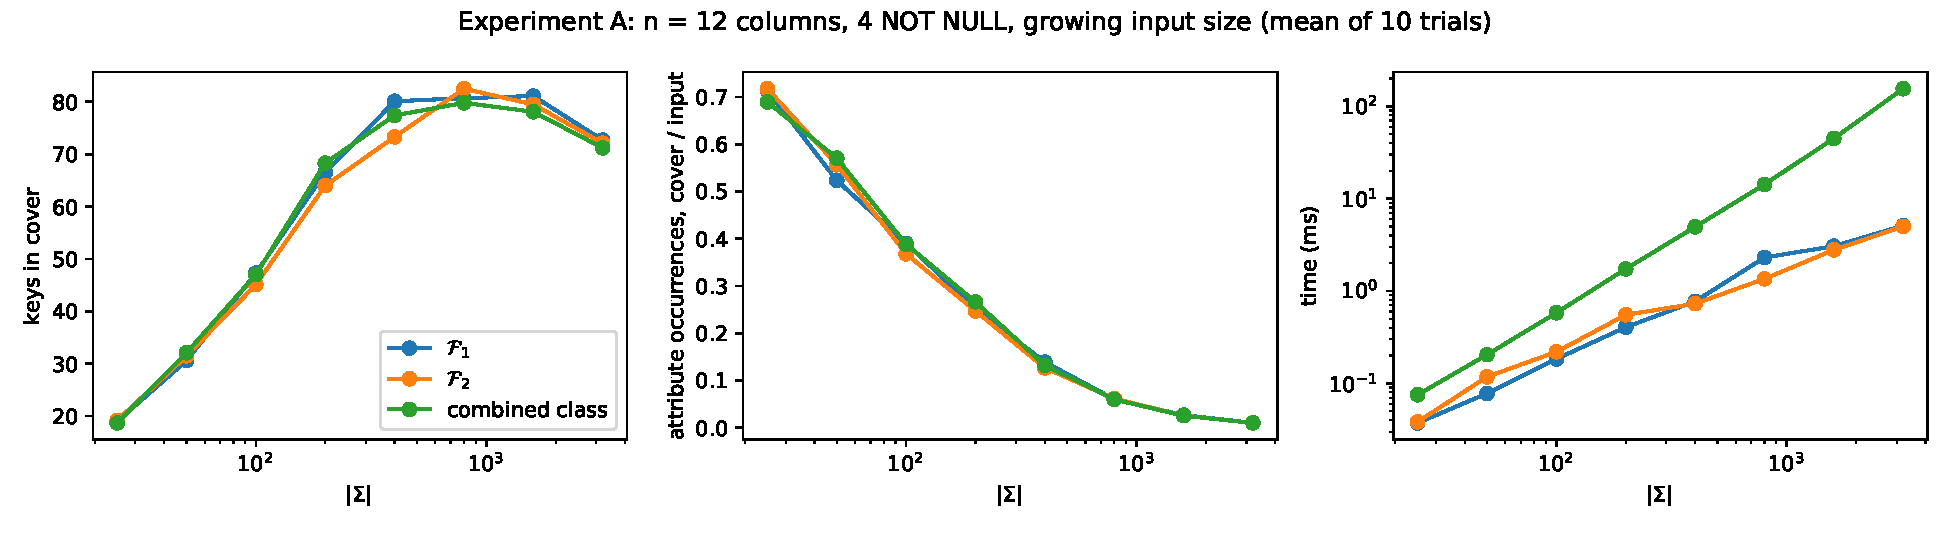
\includegraphics[width=0.9\textwidth]{figs/expA.pdf}
\caption{Experiment A: $n=12$ columns, 4 \sql{NOT NULL}, input size growing from 25
to 3200 random keys. Cover size (left), attribute occurrences of the cover relative
to the input (middle), running time (right).}
\label{fig:expA}
\Description{}
\end{figure*}

\subsection{Experiment C: partial keys against certain keys}\label{app:expC}

The hypergraph criterion of Theorem~\ref{thm:certain} is the only place where the
combined class behaves differently from its fragments, and random inputs rarely
exercise it. Experiment~C does: over $n=16$ nullable columns we draw 50 random
certain keys of 4 to 8 columns and add $p$ random \emph{binary} partial keys,
$p=0,10,\dots,120$, i.e.\ a random graph on the 16 columns with $p$ edges.
Figure~\ref{fig:expC} shows how many of the 50 certain keys survive in the cover.
With no partial keys, 44 survive (the others contain a smaller certain key). With
40 edges, a random graph on 16 vertices is already non-bipartite inside most
6-column sets, and only 25 survive; with 60 edges, 11; with 120 edges, none: every
certain key is implied by the odd cycles among its partial keys, and the cover
consists of the $p$ binary partial keys alone. Each certain key costs an index
family of size $2^{|N_K|}$ (Section~\ref{sec:indexing}), so this is where the
general cover algorithm pays off most, and it does so in $1$--$4$\,ms for the whole
input, because each colouring test is a bipartiteness check on at most 8 vertices.


\begin{figure}[t]
\centering
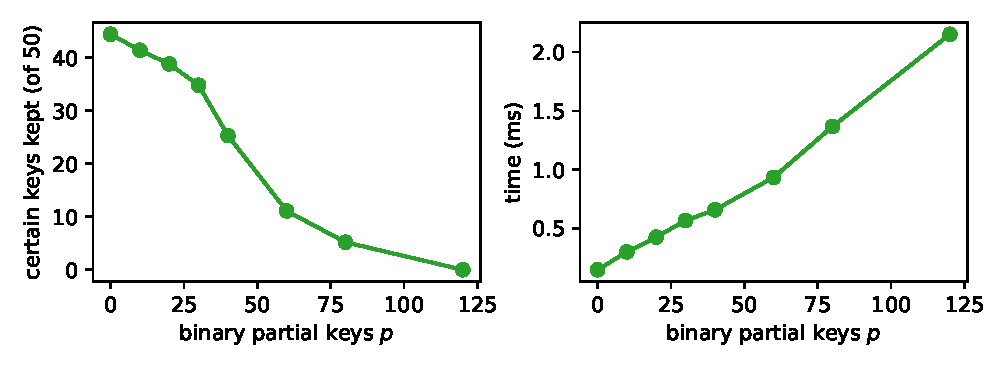
\includegraphics[width=\columnwidth]{figs/expC_col.pdf}
\caption{Experiment C: 16 nullable columns, 50 random certain keys of 4--8 columns
plus $p$ random binary partial keys: certain keys surviving in the cover (left),
running time (right).}
\label{fig:expC}
\Description{}
\end{figure}

Experiment~B (Appendix~\ref{app:expB}) grows the schema from 8 to 32 columns at
$|\Sig|=200$: random keys over many columns rarely nest, so the cover keeps 12\,\%
of the input at $n=8$ but 98\,\% at $n=32$, and the running time stays below
7\,ms.

\subsection{Experiment D: enforcement in a database}

To measure what a cover saves at run time, we enforced the input $\Sig$ and its
cover $\Gamma$ with the index scheme of Section~\ref{sec:indexing} and ran
identical workloads against both.

\paragraph{Enforcement.} The scheme is implemented exactly as described in
Section~\ref{sec:indexing}. A possible key is a \sql{UNIQUE} index (nulls
distinct). A domain key is a unique index with nulls not distinct. A partial or
certain key on $K$ with nullable part $N_K$ gets one filtered unique index per
null pattern $P\subseteq N_K$,
\begin{align*}
&\sql{CREATE UNIQUE INDEX ON T}(K\setminus P)\\
&\quad\sql{WHERE}\ \textstyle\bigwedge_{A\in P}A\ \sql{IS NULL}\ \wedge\ \bigwedge_{A\in N_K\setminus P}A\ \sql{IS NOT NULL},
\end{align*}
which rejects two records of the same pattern that agree elsewhere, plus a
\sql{BEFORE INSERT OR UPDATE} trigger that branches on the null pattern $P$ of
the new record and probes, with pure equality conditions on $K\setminus(P\cup
P')$, the index of every pattern $P'$ comparable with $P$ (partial keys) or of
every pattern $P'$ (certain keys). The experiment generates this schema in two
dialects. The PostgreSQL version uses \sql{UNIQUE NULLS NOT DISTINCT} for domain
keys, partial indexes, and one PL/pgSQL trigger function per key with the
pattern branches as \sql{IF} statements; the scripts for every configuration are
in \texttt{experiments/pg/}. The SQLite version (SQLite~3.45 in memory) realises the same scheme with
expression indexes on $\sql{coalesce}(A,-1)$ for domain keys, partial indexes,
and one trigger per null pattern whose \sql{WHEN} clause contains the probes.
We ran the experiment on both systems: the SQLite run is reported first, and the
PostgreSQL run (PostgreSQL~16.15, the generated scripts executed through
\texttt{psycopg2}) at the end of this section. Before the experiment the scheme was validated
against a brute-force implementation of Definition~\ref{def:keys} on random
instances for inserts and updates: both accepted exactly the same statements.

\paragraph{Workload and validation.} For each fragment and each
$|\Sig|\in\{10,20,40,80,120\}$ we draw $\Sig$ as in Experiment~A with keys of
at most five columns, compute $\Gamma$, and run 1500 inserts of random rows
(values uniform in $[0,200)$; with probability $0.3$ a row has a null in one
random nullable column) followed by 600 random single-column updates, accepting
or rejecting each statement by the constraints. We then run an integrity check:
for every key of the constraint set a self-join query that searches for a
violating pair (the pair conditions of Lemma~\ref{lem:typing} in SQL). In every
one of the 75 runs, on SQLite as well as on PostgreSQL, the two databases
accepted exactly the same statements and ended in the same state, which is an
end-to-end confirmation, on data, that the cover is equivalent to its input.
Moreover, the two systems accepted exactly the same statements as each other in
every run, so the SQLite emulation of \sql{NULLS NOT DISTINCT} and of the
pattern-dispatched triggers agrees with the native PostgreSQL implementation.



\begin{figure*}[t]
\centering
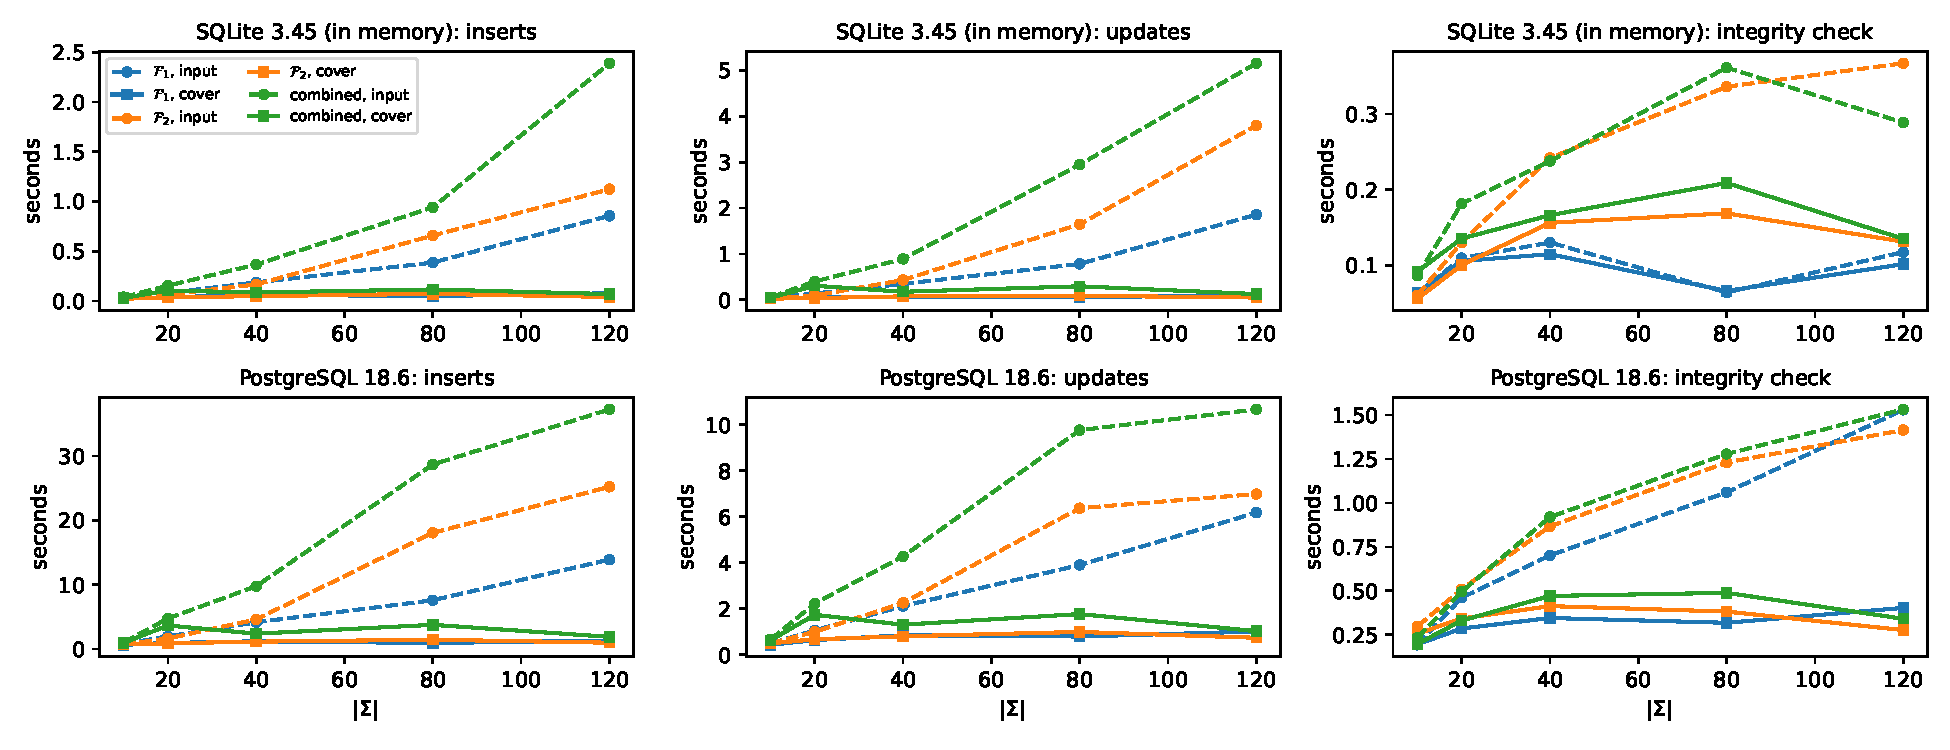
\includegraphics[width=0.9\textwidth]{figs/expD_both.pdf}
\caption{Experiment D on SQLite (top) and PostgreSQL (bottom): seconds for 1500
inserts, 600 updates and the integrity check, enforcing the input (dashed) and its
cover (solid); means of 5 runs.}
\label{fig:expDboth}
\Description{}
\end{figure*}

\begin{table}[t]
\centering
\caption{Experiment D: cover size, indexes of input and cover, and speed-up
(input time / cover time) on SQLite and PostgreSQL, means of 5 runs. Absolute
times are in Tables~\ref{tab:expD} and~\ref{tab:expDpg} (Appendix~\ref{app:expB}).}
\label{tab:expDratio}
\small
\adjustbox{max width=\columnwidth}{\begin{tabular}{l r r r r r r r r r r}
\toprule
 & & & \multicolumn{2}{c}{indexes} & \multicolumn{3}{c}{SQLite} & \multicolumn{3}{c}{PostgreSQL} \\
\cmidrule(lr){4-5}\cmidrule(lr){6-8}\cmidrule(lr){9-11}
 & $|\Sig|$ & $|\Gamma|$ & $\Sig$ & $\Gamma$ & ins & upd & chk & ins & upd & chk \\
\midrule
$\mathcal F_1$ & 10 & 7.4 & 38 & 31 & 1.4 & 1.3 & 1.0 & 1.1 & 1.1 & 3 \\
 & 40 & 16.8 & 154 & 63 & 3.7 & 4.3 & 1.2 & 4.1 & 2.9 & 4 \\
 & 120 & 27.0 & 392 & 84 & 14.5 & 13.1 & 1.4 & 13.3 & 7.0 & 84 \\
$\mathcal F_2$ & 10 & 8.0 & 27 & 25 & 1.1 & 1.0 & 1.2 & 1.1 & 1.2 & 1 \\
 & 40 & 18.4 & 128 & 54 & 4.0 & 5.4 & 1.9 & 4.7 & 3.2 & 3 \\
 & 120 & 19.8 & 421 & 55 & 35.0 & 47.4 & 3.6 & 31.7 & 9.9 & 160 \\
combined & 10 & 7.2 & 42 & 34 & 1.6 & 1.2 & 0.9 & 1.0 & 1.1 & 1 \\
 & 40 & 17.4 & 219 & 83 & 5.1 & 4.9 & 1.4 & 4.2 & 3.3 & 4 \\
 & 120 & 26.6 & 565 & 92 & 35.8 & 36.0 & 2.6 & 22.2 & 10.6 & 141 \\
\bottomrule
\end{tabular}}
\end{table}

\paragraph{Results on SQLite.} Figure~\ref{fig:expDboth} and
Table~\ref{tab:expDratio} summarise both engines. The number of indexes is the dominant quantity: every partial or certain
key costs $2^{|N_K|}$ filtered indexes and as many trigger probes, so the input
at $|\Sig|=120$ creates 390--570 indexes and 600--1000 trigger probes, the cover
55--90 indexes and 95--165 probes. Accordingly the cost of enforcing the input
grows superlinearly with $|\Sig|$, while the cost of the cover stays flat once
$|\Gamma|$ saturates at 20--27 keys. At $|\Sig|=120$ the cover makes inserts
15 times faster in $\mathcal F_1$, 35 times in $\mathcal F_2$ and 36 times in the
combined class, updates 13, 47 and 36 times faster, and the integrity check 1.4,
3.6 and 2.6 times faster; at $|\Sig|=10$ the difference is within noise, as
about 75\,\% of the keys are then non-redundant. The integrity check gains less
because the self-join per key is cheap compared to the per-statement probes and
because the check for a certain key, which dominates in $\mathcal F_2$, cannot use
an equality index on the null-bearing columns in either case. \paragraph{Results on PostgreSQL.} The second row of Figure~\ref{fig:expDboth}
and the right half of Table~\ref{tab:expDratio} report the same workload on
PostgreSQL~16 with native \sql{NULLS NOT DISTINCT} indexes, partial unique indexes
and one PL/pgSQL trigger per partial or certain key, each run one transaction with
a savepoint per statement. Times are larger than in-process SQLite, but the picture
is the same: at $|\Sig|=120$ the cover makes inserts 13, 32 and 22 times faster and
updates 7, 10 and 11 times faster, and at $|\Sig|=10$ the difference is within
noise. The integrity check gains 84--160 times, for a reason that is not execution
but planning: PostgreSQL considers every index when planning, and the self-join of
a key check on a table with 400--600 partial indexes takes 2.4\,s to plan and
0.08\,ms to execute. Every operation that touches the catalogue is thus charged for
the size of the declared key set (Experiment~F returns to this).

\paragraph{Naive enforcement.} The gain does not depend on the index scheme. With
no indexes and one trigger per key whose body is a single \sql{EXISTS} with the
pair condition of Lemma~\ref{lem:typing} (combined class, first key set of each
size), inserts took 2.0, 18.5 and 66.3\,s for the input against 1.4, 7.9 and
21.4\,s for the cover at $|\Sig|=10,40,120$, and updates 3.9, 34.9 and 157\,s
against 2.3, 14.5 and 43.5\,s: gains of 1.4--3.1 and 1.7--3.6 times, smaller than
with filtered indexes because a naive trigger costs the same for every key. On
1500 rows the naive input even beats the indexed input at $|\Sig|=120$ (66 against
128\,s), but the naive cover is four times slower than the indexed cover (21
against 5.7\,s), and naive cost grows linearly with the table.

\subsection{Experiment E: keys mined from a real database}\label{sec:expE}

The previous experiments use random key sets. To see whether declared keys are
redundant in practice we take the keys that key mining produces for a real
database: all minimal keys of every class with up to five columns, mined from the
21 tables of the Hockey database with the orthogonal key miner
of~\cite{KoehlerL25} at completeness threshold 0, at two settings of its
orthogonality filter. Level~1 is the laxest and returns 4349 possible, 118
domain, 153 partial and 187 certain keys; level~9 is the strictest and returns
only the keys the miner considers meaningful, 170 possible, 34 domain, 34 partial
and 34 certain keys. This is the standard setting of key discovery: each class is
mined on its own and returns its own minimal keys that pass the filter, so the
stock a data engineer receives is the union of four lists. Keys filtered out
would only add redundancy. Table~\ref{tab:expE} reports, per table for
level~1 and in aggregate for both levels, the declared keys by class, the cover
computed by Algorithm~\ref{alg:cover-general}, and the number of indexes of
Section~\ref{sec:indexing} that input and cover require ($2^{|N_K|}$ filtered
indexes for a partial or certain key, one per null pattern of its nullable
columns; one index otherwise). The table first takes $\NN=\emptyset$; the
effect of the profiled \sql{NOT NULL} columns is examined below.

\paragraph{Level 1.} Of the 4811 declared keys, 308 are redundant, all of one
kind: a column set mined as a minimal key of two or more classes, where only the
strongest class is needed (R1). Nothing was removed by enlargement alone (R2) or by
the colouring criterion of Theorem~\ref{thm:certain}(iii). On \textsc{Master}, the table with the most partial keys, all six
mined partial keys contain both nullable identifiers $\mathit{playerID}$ and
$\mathit{coachID}$; colouring one red and the other blue makes every edge
bichromatic, so no set of these keys implies any certain key, as an exhaustive
check over all 1023 column sets confirms. Mined minimal partial keys share their
table's identifiers in this way, whereas the colouring criterion needs small
partial keys around a cycle of alternative identifiers, as in Experiment~C; on a
second database, below, that shape does occur. Among the three classes that identify every record---domain,
partial and certain---461 are declared and 237 remain, so per-class mining doubles
the stock, and their indexes fall from 6275 to 3981. The possible keys are
a different story: \textsc{TeamSplits} alone has 3705, almost all on sparse columns
whose few non-null values happen to be distinct; these are accidental in the sense
of~\cite{KoehlerL25}, and the cover rightly keeps them, since nothing implies them.
Excluding \textsc{TeamSplits}, 28\% of the declared keys and 34\% of the
indexes are redundant.

\paragraph{Level 9.} The strict filter removes the accidental keys of the three
record-identifying classes entirely: the domain, partial and certain lists are now
the same 34 column sets, so each meaningful key is declared three times and the
cover keeps one, a certain key, in every case; the 102 declared keys of these
classes reduce to 34 and their indexes from 342 to 154. Over all four
classes 273 keys reduce to 171 (37\%) and 513 indexes to 291 (43\%). The
possible keys that survive the filter are still mostly accidental
(\textsc{TeamSplits} keeps 95 of them, pairs of columns for September games that
are null in all but a few rows), and they remain in the cover for the same reason
as before.

\paragraph{A second database.} On the VOC database of Dutch East India Company
voyages, the 239 keys mined at level~1 reduce to 175, all by R1. There the colouring shape
does occur: with $\mathit{number}$ \sql{NOT NULL}, the mined partial keys on
$\mathit{number}$ plus any two of $\mathit{yard}$, $\mathit{arrival\_date}$ and
$\mathit{next\_voyage}$ form a triangle and imply the certain key on all four
columns, which none implies alone; but a mined certain key on
$\{\mathit{number},\mathit{yard},\mathit{next\_voyage}\}$ already implies it by R2,
so the cover removes nothing by colouring.

\paragraph{\sql{NOT NULL}.} With $\NN$ set to the columns the profiles show without
nulls, the covers do not change---R1 already determines them---but their cost
does: each of the 34 meaningful certain keys of level~9 lies on \sql{NOT NULL}
columns, is a candidate key (R3), and costs one \sql{UNIQUE} index, so input and
cover cost 273 and 171 indexes. At level~1 the indexes fall from 10625 to 5277 for
the input and from 8247 to 4848 for the cover. All covers take 1.5\,s to compute
at level~1 and 1\,ms at level~9.

\paragraph{Enforcing the mined keys on the real tables.} We loaded the 20 fully
exported tables (24{,}492 rows, values pseudonymised by hashing, which preserves
equality and nulls) into PostgreSQL with their profiled \sql{NOT NULL} columns,
enforced the mined keys or their cover with the scheme of
Section~\ref{sec:indexing}, and inserted each table's own rows. Both sets accept
every row. At level~1 the cover needs 4847 instead of 5276 indexes and 125 instead
of 188 triggers, and the inserts take 178 instead of 246\,s; without
\textsc{TeamSplits}, whose 3705 accidental possible keys are all kept, the cover
removes 27\,\% of the indexes and 38\,\% of the insert time. On \textsc{Teams}, 61
partial keys on the column sets of certain keys each carried a trigger and an
index family; removing them halves the insert time (132 against 67\,s). At level~9
the cover cuts 273 \sql{UNIQUE} indexes to 171 and their storage from 11.6 to
8.3\,MiB. On VOC the cover saves 28\,\% of the indexes and 39\,\% of the insert time
(13.0 against 21.2\,s).

\paragraph{What the saving is, physically.} A possible key on $K$ is a plain
\sql{UNIQUE}$(K)$, a domain key \sql{UNIQUE}$(K)$ \sql{NULLS NOT DISTINCT}, a
certain key a family of filtered indexes: different physical objects, which
PostgreSQL builds and maintains side by side if all are declared. Only the
implication theory knows that $\ck K$ makes the other two redundant, and dropping
them is safe because the certain key's indexes reject every pair they forbid, as
the identical data admitted in Experiment~D confirms. That these removals are all
there is to gain is Theorem~\ref{thm:cover-general}: no set of keys enforces the
same constraints with fewer keys or attribute occurrences.


\begin{table}[t]
\centering
\caption{Experiment E: keys mined from the Hockey database: the ten largest tables
at orthogonality level~1, and aggregates for levels~1 and~9. Declared keys
(possible/domain/partial/certain), cover, and number of indexes of input and cover
with $\NN=\emptyset$ and of the cover with the profiled \sql{NOT NULL} columns.}
\label{tab:expE}
\small
\adjustbox{max width=\columnwidth}{\begin{tabular}{l r l r r r r}
\toprule
 & & & & \multicolumn{3}{c}{indexes} \\ \cmidrule(lr){5-7}
Table & $|\Sig|$ & by class & $|\Gamma|$ & $\Sig$ & $\Gamma$ & $\Gamma$, \sql{NN} \\
\midrule
TeamSplits & 3708 & 3705/1/1/1 & 3705 & 3714 & 3708 & 3705 \\
Master & 322 & 286/30/6/0 & 321 & 484 & 483 & 403 \\
Teams & 287 & 112/5/63/107 & 218 & 4717 & 3113 & 456 \\
Goalies & 168 & 146/6/11/5 & 152 & 392 & 309 & 174 \\
GoaliesSC & 72 & 18/18/18/18 & 18 & 356 & 160 & 18 \\
CombinedShutouts & 56 & 14/14/14/14 & 14 & 204 & 88 & 14 \\
TeamsHalf & 56 & 14/14/14/14 & 14 & 284 & 128 & 14 \\
TeamsSC & 37 & 13/10/7/7 & 16 & 103 & 49 & 16 \\
SeriesPost & 24 & 7/5/5/7 & 9 & 156 & 106 & 11 \\
Coaches & 22 & 17/3/1/1 & 17 & 36 & 24 & 17 \\
11 smaller tables & 59 & 18/13/14/14 & 19 & 179 & 79 & 20 \\
\midrule
level 1, all tables & 4811 & 4349/118/153/187 & 4503 & 10625 & 8247 & 4848 \\
\quad domain/partial/certain & 461 & 0/118/153/187 & 237 & 6275 & 3981 & \\
level 9, all tables & 273 & 170/34/34/34 & 171 & 513 & 291 & 171 \\
\quad domain/partial/certain & 102 & 0/34/34/34 & 34 & 342 & 154 & 34 \\
\bottomrule
\end{tabular}}
\end{table}


\subsection{Experiment F: query optimisation}\label{sec:expF}

We measured the rewrites of Section~\ref{sec:qopt} on the real tables of
Experiment~E in PostgreSQL, each with its \sql{NOT NULL} columns and the unique
indexes of its cover. Each query is compared with the form an optimiser reasoning
from the cover could produce, or with the same query without the key; results are
identical, the rewrites were applied by hand, and times are medians of nine runs
(Table~\ref{tab:expF}).

\paragraph{Correctness.} {\sloppy An idempotent reload of the VOC invoices with
\sql{INSERT} \dots\ \sql{ON CONFLICT (number, chamber)} \sql{DO NOTHING} inserts a
duplicate under a plain \sql{UNIQUE} index---the one invoice with a null chamber
never conflicts---and nothing under the domain key's \sql{NULLS NOT DISTINCT}
index: here \sql{UNIQUE} is wrong, not merely slow.\par}

\paragraph{Rewrites.} PostgreSQL already removes a left join through the cover's
\sql{UNIQUE} index of a possible key. It does not drop a \sql{GROUP BY} or a
\sql{DISTINCT} licensed by a domain key---for the \sql{DISTINCT} on \textsc{Master}
the key is not even in the cover but implied by its partial key (R1)---nor an
anti-join that removes subsumed records under a partial key; these rewrites make
execution 3.3 to 8.5 times faster. The certain key buys no speed for record
linkage, as the hash join is already cheap; its value is the cardinality estimate,
6136 rows instead of 367.

\begin{table}[t]
\centering
\caption{Experiment F: execution time (ms) without the key or rewrite, and with it}
\label{tab:expF}
\small
\adjustbox{max width=\columnwidth}{\begin{tabular}{l l r r r}
\toprule
Query & key & without & with & gain \\
\midrule
join removal (\textsc{Coaches}) & possible & 1.46 & 0.16 & 9.1 \\
\sql{GROUP BY} removal (invoices) & domain & 2.06 & 0.43 & 4.8 \\
\sql{DISTINCT} removal (\textsc{Master}) & domain, implied & 3.67 & 1.11 & 3.3 \\
subsumption anti-join (voyages) & partial & 6.09 & 0.72 & 8.5 \\
lookup: ship never arrived & partial & 0.95 & 0.011 & 86 \\
record linkage, one match & certain & 5.06 & 13.8 & 0.4 \\
\bottomrule
\end{tabular}}
\end{table}

\paragraph{Planning cost.} For the two self-joins over \textsc{voyages}, PostgreSQL
explores combinations of partial indexes: planning takes 0.16\,ms without indexes,
231\,ms with the cover's 157 indexes and 389\,ms with the 202 of all mined keys, for
5\,ms of execution. The cover halves the planning cost, as it did for the integrity
check of Experiment~D.

\paragraph{Hidden uniqueness.} PostgreSQL proves uniqueness only from unconditional
unique indexes. On \textsc{voyages} the cover drops
$\pos{\mathit{number},\mathit{boatname}}$, implied by
$\ck{\mathit{number},\mathit{boatname}}$, whose indexes are filtered, and the join
of a voyage with its ship's next voyage loses join removal, which a plain
\sql{UNIQUE} index restores (1.0 against 4.3\,ms). The certain key's
all-non-null index would suffice, since \sql{=} never matches null; a planner need
only accept it as a uniqueness proof. The cover is the smallest set of constraints
to enforce, not a physical design, and a designer may still add indexes for queries.
Native support for partial and certain keys would remove both this effect and the
planning overhead.

\paragraph{Summary.} Covers of thousands of keys take milliseconds, and the
colouring test removes certain keys wholesale once binary partial keys accumulate.
Enforcing the cover makes inserts, updates and integrity checks one to two orders
of magnitude faster at 120 declared keys on two systems. On keys mined from two real
databases a third to a half of the record-identifying keys are redundant, and
enforcing the cover on the real tables saves 27--28\,\% of the indexes and
38--39\,\% of the insert time; its keys also license query rewrites that SQL's
\sql{UNIQUE} does not.

%=====================================================================

\section{Related Work}\label{sec:related}
%=====================================================================

\paragraph{Keys over incomplete relations.} Keys with nulls go back to Thalheim's
key sets~\cite{Thalheim89} and the Codd families of~\cite{HLL11}; key sets were
axiomatised and their implication problem settled in~\cite{HLL23}. Possible and
certain keys, their axiomatisation and their enforcement by indexes were studied
in~\cite{KLZ15,KLLZ16}; our R1--R3 specialise to their system. Partial keys, the
ordering of the four null semantics that this paper axiomatises, and the use of
domain semantics as the default of key discovery are from~\cite{KoehlerL25}, whose
concern is the discovery of meaningful keys from inconsistent and incomplete
relations. Embedded uniqueness constraints~\cite{WLL19} add a completeness requirement to a
possible key; probabilistic and possibilistic keys~\cite{BL17,BJKLLP19} add degrees
of certainty.

\paragraph{Key discovery.} The stock of declared keys that our covers reduce is
typically produced by discovery algorithms: row-based~\cite{SBHR06}, column-based
\cite{AN11,HQAJN13} and hybrid~\cite{PN17,BBFNPS20} algorithms for unique column
combinations, which treat nulls as values, and the certain-key and
orthogonal-key miners of~\cite{KLZ16,KoehlerL25}. Discovery of approximate
constraints~\cite{KM92,PAN19,LHIK20} returns keys that almost hold and widens the
stock further. Each class is mined on its own; Experiment~E shows that the union of the outputs
is far from non-redundant.

\paragraph{Covers and physical design.} Minimal and optimal covers of functional
dependencies are due to Maier~\cite{Maier80}, who showed that optimal covers are
NP-hard to find; for keys over complete relations both notions are trivial, and
the content of Section~\ref{sec:covers} is that they remain unique when nulls split
the notion of key into five. Redundant keys are a cost in physical design: every
declared key is a candidate index for index-selection tools~\cite{CN97}, and the
index families of Section~\ref{sec:indexing} multiply that cost by $2^{|N_K|}$. Index advisors also drop duplicate indexes, but by comparing index
definitions; they cannot detect cross-class redundancy, since the filtered-index
family of a certain key and the plain \sql{UNIQUE} index of a possible key on the
same columns are different definitions. A canonical cover is also the natural input
for semantic query optimisation, which uses declared uniqueness to remove duplicate
elimination or to simplify joins~\cite{CGM90,PL94}; with nulls, which class of key
justifies which rewrite is again an implication question.
Ranking discovered keys by usefulness~\cite{PN17b,JN20} is orthogonal to a cover,
which removes only keys the others already enforce.

\paragraph{Axiomatisability.} Two-tuple witnesses and column typings are in the
spirit of Armstrong-relation constructions. Classical non-finite axiomatisability
results, for embedded multivalued dependencies or for functional with inclusion
dependencies, rest on unbounded chains; ours rests on a colouring property (see
after Theorem~\ref{thm:nonfinite}). The hardness of hypergraph 2-colourability is
due to Lov\'asz~\cite{Lovasz73}.


\section{Conclusion}\label{sec:conclusion}
%=====================================================================

The hierarchy of keys over incomplete relations~\cite{KoehlerL25} has a clean implication theory on four of its
five levels and a combinatorial one on the fifth. Certain keys are implied by partial keys exactly when a hypergraph on the
nullable columns is not 2-colourable, which rules out any finite axiomatisation and
makes implication coNP-complete, while every fragment lacking partial or certain keys
stays finitely axiomatisable and tractable. Since the cover is unique, one colouring test per declared certain key is all that stands
between a schema and the smallest set of indexes that enforces it.

Open questions include implication for key sets~\cite{Thalheim89,HLL23}
and under completeness thresholds, and an optimiser that reasons from the cover;
native support for partial and certain keys would remove the planning overhead of
filtered indexes and the uniqueness they hide (Section~\ref{sec:expF}).

Diverse ways to identify objects uniquely, but a unique way to enforce them all.


\balance
\begin{thebibliography}{10}
\bibitem{Codd70} E.~F. Codd. A relational model of data for large shared data banks.
  \emph{Commun. ACM} 13(6):377--387, 1970.
\bibitem{DD97} C.~J. Date, H. Darwen. \emph{A Guide to the SQL Standard}, 4th ed.
  Addison-Wesley, 1997.
\bibitem{Fagin81} R. Fagin. A normal form for relational databases that is based on
  domains and keys. \emph{ACM Trans. Database Syst.} 6(3):387--415, 1981.
\bibitem{GJ79} M.~R. Garey, D.~S. Johnson. \emph{Computers and Intractability}. W.~H.
  Freeman, 1979.
\bibitem{HLL11} S. Hartmann, U. Leck, S. Link. On Codd families of keys over
  incomplete relations. \emph{Comput. J.} 54(7):1166--1180, 2011.
\bibitem{HLL23} M. Hannula, X. Li, S. Link. Controlling entity integrity with key
  sets. \emph{J. Comput. Syst. Sci.} 136:195--219, 2023.
\bibitem{KLZ15} H. K\"ohler, S. Link, X. Zhou. Possible and certain SQL keys.
  \emph{Proc. VLDB Endow.} 8(11):1118--1129, 2015.
\bibitem{KLLZ16} H. K\"ohler, U. Leck, S. Link, X. Zhou. Possible and certain keys
  for SQL. \emph{VLDB J.} 25(4):571--596, 2016.
\bibitem{Lovasz73} L. Lov\'asz. Coverings and colorings of hypergraphs. In
  \emph{Proc. 4th Southeastern Conf. on Combinatorics, Graph Theory and Computing},
  pp.~3--12, 1973.
\bibitem{LO78} C.~L. Lucchesi, S.~L. Osborn. Candidate keys for relations.
  \emph{J. Comput. Syst. Sci.} 17(2):270--279, 1978.
\bibitem{KoehlerL25} H. Koehler, S. Link. Orthogonal keys: High precision and recall
  for mining database keys from inconsistent and incomplete relations.
  \emph{IEEE Trans. Knowl. Data Eng.} 37(11):6550--6561, 2025.
\bibitem{Thalheim89} B. Thalheim. On semantic issues connected with keys in
  relational databases permitting null values. \emph{J. Inf. Process. Cybern.}
  25(1/2):11--20, 1989.
\bibitem{ZL25} Z. Zhang, S. Link. Mixed covers: optimizing updates and queries using
  minimal keys and functional dependencies. \emph{VLDB J.} 34(3):29, 2025.
\bibitem{WLL19} Z. Wei, U. Leck, S. Link. Discovery and ranking of embedded uniqueness
  constraints. \emph{Proc. VLDB Endow.} 12(13):2339--2352, 2019.
\bibitem{BL17} P. Brown, S. Link. Probabilistic keys. \emph{IEEE Trans. Knowl. Data
  Eng.} 29(3):670--682, 2017.
\bibitem{BJKLLP19} N. Balamuralikrishna, Y. Jiang, H. Koehler, U. Leck, S. Link, H. Prade.
  Possibilistic keys. \emph{Fuzzy Sets Syst.} 376:1--36, 2019.
\bibitem{SBHR06} Y. Sismanis, P. Brown, P. J. Haas, B. Reinwald. GORDIAN: efficient and
  scalable discovery of composite keys. In \emph{VLDB}, pp. 691--702, 2006.
\bibitem{AN11} Z. Abedjan, F. Naumann. Advancing the discovery of unique column
  combinations. In \emph{CIKM}, pp. 1565--1570, 2011.
\bibitem{HQAJN13} A. Heise, J. Quian\'e-Ruiz, Z. Abedjan, A. Jentzsch, F. Naumann.
  Scalable discovery of unique column combinations. \emph{Proc. VLDB Endow.}
  7(4):301--312, 2013.
\bibitem{PN17} T. Papenbrock, F. Naumann. A hybrid approach for efficient unique column
  combination discovery. In \emph{BTW}, LNI P-265, pp. 195--204, 2017.
\bibitem{BBFNPS20} J. Birnick, T. Bl\"asius, T. Friedrich, F. Naumann, T. Papenbrock,
  M. Schirneck. Hitting set enumeration with partial information for unique column
  combination discovery. \emph{Proc. VLDB Endow.} 13(11):2270--2283, 2020.
\bibitem{KLZ16} H. K\"ohler, S. Link, X. Zhou. Discovering meaningful certain keys from
  incomplete and inconsistent relations. \emph{IEEE Data Eng. Bull.} 39(2):21--37, 2016.
\bibitem{KM92} J. Kivinen, H. Mannila. Approximate dependency inference from
  relations. In \emph{ICDT}, LNCS 646, pp. 86--98, 1992.
\bibitem{PAN19} E. H. M. Pena, E. C. de Almeida, F. Naumann. Discovery of approximate
  (and exact) denial constraints. \emph{Proc. VLDB Endow.} 13(3):266--278, 2019.
\bibitem{LHIK20} E. Livshits, A. Heidari, I. F. Ilyas, B. Kimelfeld. Approximate denial
  constraints. \emph{Proc. VLDB Endow.} 13(10):1682--1695, 2020.
\bibitem{Maier80} D. Maier. Minimum covers in the relational database model.
  \emph{J. ACM} 27(4):664--674, 1980.
\bibitem{CN97} S. Chaudhuri, V. R. Narasayya. An efficient cost-driven index selection
  tool for Microsoft SQL Server. In \emph{VLDB}, pp. 146--155, 1997.
\bibitem{PN17b} T. Papenbrock, F. Naumann. Data-driven schema normalization. In
  \emph{EDBT}, pp. 342--353, 2017.
\bibitem{JN20} L. Jiang, F. Naumann. Holistic primary key and foreign key detection.
  \emph{J. Intell. Inf. Syst.} 54(3):439--461, 2020.
\bibitem{OracleDoc} Oracle. \emph{Database Concepts}, chapter Indexes and
  Index-Organized Tables. \url{https://docs.oracle.com/en/database/oracle/oracle-database/}, accessed 2026.
\bibitem{SQLServerDoc} Microsoft. \emph{SQL Server documentation}: Unique constraints
  and check constraints; Create filtered indexes. \url{https://learn.microsoft.com/sql/}, accessed 2026.
\bibitem{PGDoc} PostgreSQL Global Development Group. \emph{PostgreSQL 15 Release
  Notes} and \emph{Documentation}: CREATE INDEX; Partial indexes.
  \url{https://www.postgresql.org/docs/15/}, accessed 2026.
\bibitem{Db2Doc} IBM. \emph{Db2 documentation}: CREATE INDEX statement.
  \url{https://www.ibm.com/docs/en/db2}, accessed 2026.
\bibitem{CGM90} U. S. Chakravarthy, J. Grant, J. Minker. Logic-based approach to
  semantic query optimization. \emph{ACM Trans. Database Syst.} 15(2):162--207, 1990.
\bibitem{PL94} G. N. Paulley, P.-{\AA}. Larson. Exploiting uniqueness in query
  optimization. In \emph{ICDE}, pp. 68--79, 1994.
\bibitem{GL94} C. A. Galindo-Legaria. Outerjoins as disjunctions. In \emph{SIGMOD},
  pp. 348--358, 1994.
\bibitem{GL16} P. Guagliardo, L. Libkin. Making SQL queries correct on incomplete
  databases: a feasibility study. In \emph{PODS}, pp. 211--223, 2016.
\end{thebibliography}

\clearpage
\appendix
\section{Pairs and Types}\label{app:pairs}
%=====================================================================

Every key class constrains pairs of tuples only, which turns implication into a
question about two-tuple instances.

\begin{lemma}[Pair lemma]\label{lem:pair}
For every class $\mathcal C$ and instance $i$: $i$ satisfies $\mathcal C(K)$ iff
every two-element sub-multiset $\{t,t'\}$ of $i$ (with $t,t'$ distinct records)
satisfies $\mathcal C(K)$.
\end{lemma}
\begin{proof}
Each clause of Definition~\ref{def:keys} forbids a pair of distinct tuples with a
property of that pair alone; totality is a per-tuple condition. \end{proof}

\begin{corollary}\label{cor:pair}
$\Sig\not\models\varphi$ iff some two-tuple instance over $(S,\NN)$ satisfies
$\Sig$ and violates $\varphi$.
\end{corollary}

A two-tuple instance $\{t,t'\}$ is described by a \emph{type} $\tau(C)$ for each
column $C$, listed in Table~\ref{tab:types}. Columns in $\NN$ have type \eq\ or
\dd\ only, and every assignment of types respecting this restriction is realised by
a two-tuple instance.

\begin{table}[t]
\centering
\caption{Column types of a two-tuple instance $\{t,t'\}$, with the types of $i_0$'s
records 1 and 3 as an example}
\label{tab:types}
\adjustbox{max width=\columnwidth}{\begin{tabular}{l l l l}
\toprule
Type & $t(C)$ & $t'(C)$ & column of $(i_0$ records $1,3)$ \\
\midrule
\bn & \nul & \nul & --- \\
\eq & $v$ & $v$ (same non-null value) & --- \\
\nv & \nul & $v$ & $\mathit{DoB}$, $\mathit{Salary}$ \\
\vn & $v$ & \nul & $\mathit{Job}$ \\
\dd & $v$ & $w$ (both non-null, $v\neq w$) & $\mathit{Name}$ \\
\bottomrule
\end{tabular}}
\end{table}

\begin{lemma}[Typing lemma]\label{lem:typing}
For $L\subseteq S$, the two-tuple instance $\{t,t'\}$ satisfies
\begin{itemize}
\item $\pos{L}$ iff some $C\in L$ has $\tau(C)\neq\eq$;
\item $\dom{L}$ iff some $C\in L$ has $\tau(C)\in\{\nv,\vn,\dd\}$;
\item $\pk{L}$ iff some $C\in L$ has $\tau(C)\in\{\vn,\dd\}$ and some $C\in L$ has
  $\tau(C)\in\{\nv,\dd\}$;
\item $\ck{L}$ iff some $C\in L$ has $\tau(C)=\dd$.
\end{itemize}
\end{lemma}

\begin{example}
Records 1 and 3 of $i_0$ have the types of Table~\ref{tab:types}. By
Lemma~\ref{lem:typing} this pair satisfies $\pk{\mathit{Salary},\mathit{Job}}$
(\nv\ on $\mathit{Salary}$, \vn\ on $\mathit{Job}$) and violates
$\ck{\mathit{Salary},\mathit{Job}}$ (no \dd), as observed in Section~\ref{sec:motivation}. It
satisfies $\ck{\mathit{Name},\mathit{Job}}$ through the \dd\ column
$\mathit{Name}$.
\end{example}

The four conditions of Lemma~\ref{lem:typing} are superset-closed in $L$ and nested
in the order certain $\Rightarrow$ partial $\Rightarrow$ domain $\Rightarrow$
possible; this is the hierarchy~\eqref{eq:hierarchy} at the level of pairs, and the
types \dd, \vn, \nv, \bn\ witness its strictness in turn.

\begin{remark}\label{rem:noaxiom}
No key is valid: the two-tuple instance with every column of type \eq\ violates
$\pos{K}$ for every $K$, including $K=\emptyset$. A sound inference system therefore
has no axioms, only rules with at least one premise.
\end{remark}



\section{Further Results and Examples}\label{app:examples}

\begin{lemma}\label{lem:cycle}
\begin{enumerate}
\item[(a)] $\Sig_k\models\ck{S_k}$.
\item[(b)] For every proper subset $\Sig'\subsetneq\Sig_k$ and every $L\subseteq S_k$,
  $\Sig'\not\models\ck{L}$.
\item[(c)] For every $\Sig'\subseteq\Sig_k$, $L\subseteq S_k$ and $\mathcal C\in\{$possible,
  domain, partial$\}$: $\Sig'\models\mathcal C(L)$ iff $A_iA_{i+1}\subseteq L$ for
  some $\pk{A_iA_{i+1}}\in\Sig'$.
\end{enumerate}
\end{lemma}
\noindent\emph{Proof idea.} (a) $H(\Sig_k,S_k)$ is the odd cycle $C_{2k+1}$. (b) Removing an edge leaves a path, which is bipartite. Full proof in Appendix~\ref{app:proofs}.


\begin{corollary}[A complete infinite system]\label{cor:infinite}
R1--R4 together with the rule scheme
\[
\{\,\pk{Xe} : e\in E\,\}\ \vdash\ \ck{XA_1\cdots A_n},
\]
for $X\subseteq\NN$ and every hypergraph $(\{A_1,\dots,A_n\},E)$ with no proper 2-colouring,
is sound and complete for the combined class. It suffices to include the
edge-critical hypergraphs, those all of whose proper sub-hypergraphs are
2-colourable.
\end{corollary}
\noindent\emph{Proof idea.} Every non-2-colourable hypergraph contains an edge-critical one, whose rule derives the target; the remaining cases are Theorem~\ref{thm:complete}. Full proof in Appendix~\ref{app:proofs}.


\begin{example}
For $\Sig_0$ of Section~\ref{sec:why} and target $\pos{\mathit{Name},\mathit{DoB}}$,
the closure $\Sig_0^+$ contains no key contained in $\{\mathit{Name},\mathit{DoB}\}$,
so the theorem's \eq-instance consisting of the records
$(\text{Eve},\allowbreak 01/01/2000,\allowbreak 1\mathrm k,\allowbreak \text{A})$ and
$(\text{Eve},\allowbreak 01/01/2000,\allowbreak 2\mathrm k,\allowbreak \text{B})$ satisfies $\Sig_0$ and
violates the target: the possible key on name and date of birth is not redundant
and its \sql{UNIQUE} index must stay.
\end{example}

\begin{example}
Take $\Sig_0$ of Section~\ref{sec:why} in $\mathcal F_1$, with
$\NN=\{\mathit{Name}\}$ and the certain key replaced by its $\mathcal F_1$-analogue
$\pk{\mathit{Name},\mathit{Job}}$. After sorting, $\pos{\mathit{Job}}$ and
$\dom{\mathit{Salary}}$ enter $\Gamma$, as no key precedes them. Then
$\pk{\mathit{Salary},\mathit{Job}}$ enters, because the two keys inside it are
weaker, and so does $\pk{\mathit{Name},\mathit{Job}}$. Thus $\Sig_0$ is its own
cover. Adding $\dom{\mathit{Salary},\mathit{Job}}$ would be rejected at once by
$\pk{\mathit{Salary},\mathit{Job}}$.
\end{example}

\section{Deferred Proofs}\label{app:proofs}
\noindent\textbf{Proof of Lemma~\ref{lem:typing}.}
$\pos{L}$ fails iff both values are non-null and equal on every column of $L$, i.e.\
all types are \eq. $\dom{L}$ fails iff $t(C)=t'(C)$ on all of $L$ with $\nul=\nul$,
i.e.\ all types lie in $\{\bn,\eq\}$. $\pk{L}$ fails iff $t$ is subsumed by $t'$ on
$L$, i.e.\ all types lie in $\{\bn,\eq,\nv\}$, or $t'$ is subsumed by $t$, i.e.\ all
types lie in $\{\bn,\eq,\vn\}$; negating both disjuncts gives the stated conjunction.
$\ck{L}$ fails iff on every column of $L$ one value is null or the two agree, i.e.\
no column has type \dd. \qed

\noindent\textbf{Proof of Corollary~\ref{cor:fragments}.}
For targets other than certain keys this is Theorem~\ref{thm:complete}. For a certain
target with no partial keys among the premises, Theorem~\ref{thm:certain} below
shows that implication holds only through a certain premise contained in $K$ or a
premise contained in $K\cap\NN$, both derivable by R1--R3. \qed

\noindent\textbf{Proof of Theorem~\ref{thm:sound}.}
By Lemma~\ref{lem:pair} it suffices to consider a two-tuple instance with type
assignment $\tau$; by Lemma~\ref{lem:typing} satisfaction is read off $\tau$.

\emph{R1.} The four conditions of Lemma~\ref{lem:typing} are nested as stated; for
candidate keys use Lemma~\ref{lem:cand}.

\emph{R2.} Each condition asks for a column of some type inside the key, and is
preserved when the key grows.

\emph{R3.} If $K\subseteq\NN$ every column of $K$ has type \eq\ or \dd. $\pos{K}$
supplies a column of type other than \eq, hence \dd, hence $\ck{K}$.

\emph{R4.} $\pk{XA}$ supplies $C_1$ with $\tau(C_1)\in\{\vn,\dd\}$ and $C_2$ with
$\tau(C_2)\in\{\nv,\dd\}$. If either is \dd\ then $\ck{XA}$ holds. Otherwise
$\tau(C_1)=\vn$ and $\tau(C_2)=\nv$; columns of $X\subseteq\NN$ have neither type,
so $C_1=C_2=A$, which gives $A$ two types.

\emph{R5.} Suppose $\ck{XABC}$ fails: no column of $XABC$ has type \dd, so every
column of $X$ is \eq. For $\pk{XAB}$ to hold, $\{A,B\}$ must contain a \vn\ column
and an \nv\ column, i.e.\ $\tau(A),\tau(B)\in\{\vn,\nv\}$ with $\tau(A)\neq\tau(B)$.
Likewise for $\{A,C\}$ and $\{B,C\}$. Three columns cannot be pairwise distinct
under two types. \qed

\noindent\textbf{Proof of Theorem~\ref{thm:complete}.}
In each case we give a type assignment $\tau$, hence by Corollary~\ref{cor:pair} a
two-tuple instance over $(S,\NN)$, that violates $\varphi$ and satisfies $\Sig$. Two
conventions hold throughout: columns outside $K$ get type \dd, which by
Lemma~\ref{lem:typing} satisfies every key $\mathcal C(L)$ with $L\not\subseteq K$ in
every class; columns of $K\cap\NN$ get type \eq, admissible on \sql{NOT NULL}
columns. Only premises $\mathcal C(L)\in\Sig$ with $L\subseteq K$ need checking.

\emph{Case $\varphi=\pos{K}$.} Set $\tau(C)=\eq$ for all $C\in K$; this violates
$\pos{K}$. If $\mathcal C(L)\in\Sig$ with $L\subseteq K$ then $\mathcal C(L)\vdash
\pos{L}$ by R1 (via Lemma~\ref{lem:cand} if $\mathcal C$ is candidate) and $\pos{L}
\vdash\pos{K}$ by R2, contradicting $\pos{K}\notin\Sig^+$. So no such premise
exists.

\emph{Case $\varphi=\dom{K}$.} If $K\subseteq\NN$ then $\pos{K}\notin\Sig^+$, for
otherwise R3 and R1 give $\dom{K}\in\Sig^+$; the instance of the previous case
violates $\pos{K}$ and hence $\dom{K}$. If $K\not\subseteq\NN$ set $\tau(A)=\bn$ for
$A\in K\cap N$. No column of $K$ has type \nv, \vn\ or \dd, so $\dom{K}$ fails. Let
$\mathcal C(L)\in\Sig$ with $L\subseteq K$. If $\mathcal C$ is domain, partial,
certain or candidate then R1 and R2 put $\dom{K}$ into $\Sig^+$. If $\mathcal C$ is
possible then $\pos{L}$ holds iff $L$ has a non-\eq\ column iff $L\cap N\neq
\emptyset$; if instead $L\subseteq K\cap\NN$ then $\pos{L}\vdash\ck{L}\vdash\dom{L}
\vdash\dom{K}$ by R3, R1, R2, a contradiction.

\emph{Case $\varphi=\pk{K}$.} If $K\subseteq\NN$ argue as before with the
\eq-instance. If $K\not\subseteq\NN$ set $\tau(A)=\nv$ for $A\in K\cap N$. No column
of $K$ has type \vn\ or \dd, so $\pk{K}$ fails. Let $\mathcal C(L)\in\Sig$ with
$L\subseteq K$. If $\mathcal C$ is partial, certain or candidate then $\pk{K}\in
\Sig^+$ by R1, R2. If $\mathcal C$ is domain or possible then $\mathcal C(L)$ holds
iff $L\cap N\neq\emptyset$, since an \nv\ column satisfies both; if $L\subseteq K\cap
\NN$ then R3, R1, R2 derive $\pk{K}$, a contradiction.

\emph{Case $\varphi=\cand{K}$.} By Lemma~\ref{lem:cand}, $\Sig\models\cand{K}$ iff
$K\subseteq\NN$ and $\Sig\models\ck{K}$. If $K\not\subseteq\NN$, the one-tuple
instance with a null in $K\setminus\NN$ satisfies $\Sig$ and violates $\cand{K}$. If
$K\subseteq\NN$ then $\ck{K}\in\Sig^+$ iff $\pos{K}\in\Sig^+$ by R1 and R3, so
$\cand{K}\notin\Sig^+$ gives $\pos{K}\notin\Sig^+$ and the \eq-instance violates
$\ck{K}$, hence $\cand{K}$. \qed

\noindent\textbf{Proof of Theorem~\ref{thm:certain}.}
($\Leftarrow$) Conditions (i) and (ii) give $\ck{K}$ by the sound rules R1, R2, R3.
For (iii), suppose a two-tuple instance $\{t,t'\}$ satisfies $\Sig$ and violates
$\ck{K}$. By Lemma~\ref{lem:typing} no column of $K$ has type \dd, and the columns of
$K\cap\NN$ have type \eq. Define $c(A):=$ red if $\tau(A)=\vn$, blue if $\tau(A)=
\nv$, and arbitrarily if $\tau(A)\in\{\bn,\eq\}$. Take any $\pk{L}\in\Sig$ with
$L\subseteq K$. Since $L$ has no \dd\ column, Lemma~\ref{lem:typing} requires a \vn\
column and an \nv\ column in $L$; both are nullable, so both lie in the edge $L\cap
N_K$, which sees both colours. Hence $c$ is proper, contradicting (iii). By
Lemma~\ref{lem:pair} no instance satisfies $\Sig$ and violates $\ck{K}$.

($\Rightarrow$) Suppose none of (i)--(iii) holds and fix a proper colouring $c$.
Define $\tau(C)=\eq$ for $C\in K\cap\NN$; $\tau(A)=\vn$ if $c(A)$ is red and
$\tau(A)=\nv$ if $c(A)$ is blue, for $A\in N_K$; and $\tau(C)=\dd$ for $C\notin K$.
No column of $K$ has type \dd, so $\ck{K}$ fails. Let $\mathcal C(L)\in\Sig$. If
$L\not\subseteq K$, the \dd\ column satisfies $\mathcal C(L)$ in every class. If
$L\subseteq K$: certain and candidate are excluded by $\neg$(i). If $\mathcal C$ is
possible or domain then $L\not\subseteq\NN$ by $\neg$(ii), so $L$ contains a nullable
column of $K$, whose mixed type satisfies both. If $\mathcal C$ is partial then
$L\cap N_K$ is an edge of $H(\Sig,K)$, hence bichromatic, so $L$ has a \vn\ and an
\nv\ column and $\pk{L}$ holds. Thus the instance satisfies $\Sig$. \qed

\noindent\textbf{Proof of Corollary~\ref{cor:infinite}.}
Soundness is the ($\Leftarrow$) direction of Theorem~\ref{thm:certain} for partial
premises. For completeness, non-certain targets are Theorem~\ref{thm:complete}; for
$\ck{K}$ with $\Sig\models\ck{K}$ one of (i)--(iii) holds, (i) and (ii) are derivable
by R1--R3, and under (iii) $H(\Sig,K)$ contains an edge-critical sub-hypergraph whose
rule, followed by R2, derives $\ck{K}$. Candidate targets reduce by
Lemma~\ref{lem:cand}. \qed

\noindent\textbf{Proof of Lemma~\ref{lem:cycle}.}
(a) $H(\Sig_k,S_k)$ is the cycle $C_{2k+1}$, which has no proper 2-colouring; apply
Theorem~\ref{thm:certain}(iii).
(b) $\Sig'$ contains no certain or candidate key, and $\NN=\emptyset$ makes (ii)
void. $H(\Sig',L)$ has edge set $\{A_iA_{i+1}\in\Sig' : A_i,A_{i+1}\in L\}$, a
subgraph of a path, hence bipartite, with all edges of size two. So (iii) fails and
Theorem~\ref{thm:certain} gives $\Sig'\not\models\ck{L}$.
(c) By Theorem~\ref{thm:complete}, $\Sig'\models\mathcal C(L)$ iff $\mathcal C(L)$
lies in the closure of $\Sig'$ under R1--R4. R3 never fires ($\NN=\emptyset$) and
R4 never fires (it needs a key with at most one nullable column, while every key of
$\Sig'$ has two and derived keys only grow). So the closure consists of the superkeys
of members of $\Sig'$ in the classes partial, domain and possible. \qed

\noindent\textbf{Proof of Theorem~\ref{thm:maximal-classes}.}
If $\{$partial, certain$\}\subseteq\mathcal F$, Theorem~\ref{thm:nonfinite} applies
verbatim, since its witnesses use only these two classes.

Otherwise, candidate keys do not disturb either fragment: by the convention of
Section~\ref{sec:prelim} a candidate premise is a certain key on \sql{NOT NULL}
columns and contributes only to condition (i) of Theorem~\ref{thm:certain}, and a
candidate target has $N_K=\emptyset$ by Lemma~\ref{lem:cand}, so condition (iii)
can hold only through the empty edge, i.e.\ through a premise contained in
$K\subseteq\NN$, which R3 and R1 derive.

For $\mathcal F_1$: the targets are possible, domain, partial or candidate keys, so
Theorem~\ref{thm:complete} applies; its proof uses R1, R2 and, for the upgrade on
total columns, only R3 followed by R1, which is the stated instance of R3. R4 is used
nowhere in that proof. For $\mathcal F_2$: for non-certain targets
Theorem~\ref{thm:complete} applies without R4, whose premise is a partial key; for a
certain target there are no partial premises, so $E=\emptyset$ in
Theorem~\ref{thm:certain} and implication holds only through conditions (i) and (ii),
which R1--R3 derive. Any set of classes not containing both partial and certain keys
is contained in $\mathcal F_1$ or $\mathcal F_2$, and both are finitely axiomatisable,
so they are the maximal ones.
\qed

\noindent\textbf{Proof of Theorem~\ref{thm:cover-frag-alg}.}
Lines~1--3 replace keys by equivalent ones and remove equivalent duplicates, so
the resulting $\Sig$ is equivalent to the input and contains no two equivalent
keys. Write $\gamma\sqsubseteq\sigma$ for the condition of line~9; by
\eqref{eq:impl-frag}, $\gamma\sqsubseteq\sigma$ iff $\{\gamma\}\models\sigma$, and
$\sqsubseteq$ is transitive. If $\gamma\sqsubseteq\sigma$ with $\gamma\neq\sigma$
then $|L|<|K|$, or $|L|=|K|$, $L=K$ and $\mathcal C'\succ\mathcal C$ (a total $L=K$
with different classes was merged in line~2), so $\gamma$ precedes $\sigma$ in the
sorted order.

\emph{Cover.} Let $\sigma\in\Sig$ be rejected at line~13. Then some $\gamma_1\in
\Gamma$ has $\gamma_1\sqsubseteq\sigma$, and $\gamma_1\in\Gamma$ at the end, so
$\Gamma\models\sigma$. Hence $\Gamma\models\Sig$; and $\Gamma\subseteq\Sig$.

\emph{Non-redundant.} Suppose $\sigma\in\Gamma$ and $\Gamma\setminus\{\sigma\}
\models\sigma$. By single-premise implication some $\gamma\in\Gamma\setminus
\{\sigma\}$ has $\gamma\sqsubseteq\sigma$, so $\gamma$ precedes $\sigma$ and was in
$\Gamma$ when $\sigma$ was examined; then $\sigma$ would have been rejected.

\emph{Complexity.} Column sets are bit vectors of $n$ bits; a subset test and a
class comparison take $O(n)$. Sorting is $O(|\Sig|\log|\Sig|\cdot n)$ with $O(n)$
comparisons of keys, and the double loop performs at most $|\Sig|\cdot|\Gamma|\le
|\Sig|^2$ tests. Space is the input plus $\Gamma$, $O(|\Sig|n)$ bits.
\qed

\noindent\textbf{Proof of Theorem~\ref{thm:cover-general}.}
Fix $\sigma=\mathcal C(K)\in\Sig$. We use two facts. (F1) For a target of class
possible, domain or partial, implication is single-premise: by
Theorem~\ref{thm:complete} and the correctness proof of Algorithm~\ref{alg:decide}
(lines~6--11), $\Delta\models\mathcal C(K)$ iff some $\mathcal C'(L)\in\Delta$ has
$L\subseteq K$ and ($\mathcal C'\succeq\mathcal C$ or $L\subseteq\NN$), and that
key alone implies $\mathcal C(K)$. (F2) For a certain target,
Theorem~\ref{thm:certain} applies.

\emph{Case $\mathcal C\preceq$ partial.} By (F1) some $\gamma=\mathcal C'(L)\in
\Gamma$ with $L\subseteq K$ implies $\sigma$. If $\gamma$ is not a certain key,
then by (F1) applied to $\Sig\models\gamma$ some $\sigma'\in\Sig$ implies $\gamma$,
hence $\sigma$; non-redundancy gives $\sigma'=\sigma$ and $\gamma\equiv\sigma$. If
$\gamma=\ck L$, apply (F2) to $\Sig\models\ck L$: under condition (i) a certain or
candidate premise $\ck M\in\Sig$ with $M\subseteq L\subseteq K$ implies $\sigma$, so
it equals $\sigma$, impossible as $\sigma$ is not certain---unless $K\subseteq\NN$,
where it means $M=K=L$ and $\gamma\equiv\sigma$; under (ii) a premise on
$M\subseteq L\cap\NN$ implies $\sigma$ by R3, so it is $\sigma$, whence $K\subseteq
\NN$, $L=K$ and $\gamma\equiv\sigma$; under (iii) there are partial premises
$\pk{M_j}\in\Sig$ with $M_j\subseteq L\subseteq K$ forming a non-2-colourable
hypergraph on $L\cap N$. Each $\pk{M_j}$ implies $\sigma$, so each equals $\sigma$:
thus $\sigma=\pk K$, $M_j=L=K$, and the hypergraph is the single edge $K\cap N$,
non-colourable only if $|K\cap N|\le1$, in which case $\gamma=\ck K\equiv\pk K=
\sigma$ by R4.

\emph{Case $\mathcal C=$ certain.} Apply (F2) to $\Gamma\models\ck K$.
(i) $\gamma=\ck L$ or $\cand L\in\Gamma$ with $L\subseteq K$. Apply (F2) to
$\Sig\models\ck L$: under (i) a certain premise $\ck M\in\Sig$, $M\subseteq L$,
implies $\sigma$, so it is $\sigma$, $L=K$, $\gamma\equiv\sigma$; under (ii) a
premise inside $L\cap\NN$ implies $\sigma$, so it is $\sigma$, $K\subseteq L$,
$L=K$, $\gamma\equiv\sigma$; under (iii) partial premises of $\Sig$ inside $L$
imply $\ck L$, hence $\Sig\setminus\{\sigma\}\models\ck K$, contradicting
non-redundancy.
(ii) $\gamma\in\Gamma$ on $L\subseteq K\cap\NN$ of any class. Then $\gamma\models
\sigma$ by R3, and $\Sig\models\gamma$; if $\gamma$ is not certain, (F1) gives
$\sigma'\in\Sig$ with $\sigma'\models\gamma\models\sigma$, so $\sigma'=\sigma$ and
$\gamma\equiv\sigma$; if $\gamma$ is certain, argue as in (i).
(iii) Partial keys $\gamma_j=\pk{L_j}\in\Gamma$, $L_j\subseteq K$, whose edges
$L_j\cap N$ form a non-2-colourable hypergraph. By (F1), $\Sig\models\pk{L_j}$ is
witnessed by a single $\sigma_j\in\Sig$ on $M_j\subseteq L_j$ that is partial or
certain, or any class with $M_j\subseteq L_j\cap\NN$. If $\sigma_j$ is certain, or
total, it implies $\ck K$, so $\sigma_j=\sigma$ and $L_j=K$. Hence the hypergraph
$E'$ consisting of $M_j\cap N$ for the $j$ with $\sigma_j\neq\sigma$ (these are
partial premises of $\Sig\setminus\{\sigma\}$) together with $K\cap N$ if some
$\sigma_j=\sigma$ refines the hypergraph of the $L_j$, so it is non-2-colourable.
If $E'' :=E'\setminus\{K\cap N\}$ is non-colourable then $\Sig\setminus\{\sigma\}
\models\ck K$, a contradiction. Otherwise $E''$ is colourable and $E'$ is not; a
proper colouring of $E''$ fails on the edge $K\cap N$ only if $K\cap N$ is
monochromatic, which for a non-empty $E''$ (whose edges lie inside $K\cap N$ and
are bichromatic) is impossible. So $E''=\emptyset$ and the single edge $K\cap N$ is
non-colourable, i.e.\ $|K\cap N|\le1$; then $\gamma_j=\pk K\equiv\ck K=\sigma$ by
R4.

In every case $\Gamma$ contains a key equivalent to $\sigma$, and the consequence
follows exactly as in Theorem~\ref{thm:cover-frag}.
\qed

\noindent\textbf{Proof of Theorem~\ref{thm:cover-general-alg}.}
Lines~1--4 replace keys by equivalent keys (Lemma~\ref{lem:cand}, R3, R4 with R1)
and remove equivalent duplicates. The loop maintains $\Gamma\equiv\Sig$: a key is
removed only when the rest implies it. At the end $\Gamma$ is non-redundant: if
$\Gamma\setminus\{\sigma\}\models\sigma$ for some $\sigma\in\Gamma$, this already
held when $\sigma$ was examined, because keys were only removed afterwards and
removal shrinks the implied set, so $\sigma$ would have been removed then. (The
descending order is not needed for correctness---by Theorem~\ref{thm:cover-general}
every removal order gives the same result up to equivalence---but it tests wide
certain keys, the most expensive ones, against the largest possible $\Gamma$ first
and tends to remove them early.)

For a non-certain $\sigma$ the test of line~8 is a scan with one subset test per
key, $O(|\Gamma|\,n)$, correct by (F1) in the proof of
Theorem~\ref{thm:cover-general}; over all non-certain keys this is $O(|\Sig|^2n)$.
For a certain $\sigma$ line~10 calls Algorithm~\ref{alg:decide}, whose cost by
Theorem~\ref{thm:algcost} is $O(|\Gamma|n+m^2n+2^{|N_K|-1}(|N_K|+m))$ with
$|N_K|\le b$; summed over the $c$ certain keys this gives the second term, and the
scan part is absorbed into $O(|\Sig|^2n)$. The space bound is that of
Algorithm~\ref{alg:decide} plus $\Gamma$. The polynomial cases are those of
Theorem~\ref{thm:algcost}.
\qed

\noindent\textbf{Proof of Theorem~\ref{thm:nonfinite}.}
Suppose such a system exists with premise bound $m$, and choose $k$ with $2k+1>m$.
By Remark~\ref{rem:noaxiom} the system has no axioms, so every derivation starts
from $\Sig_k$. Take a derivation of $\ck{S_k}$ from $\Sig_k$, which exists by
completeness and Lemma~\ref{lem:cycle}(a), and consider the first rule application
in it whose conclusion $\psi$ is a certain or a candidate key. Its premises
$\psi_1,\dots,\psi_j$ with $j\le m$ are derived earlier, so by soundness each is
implied by $\Sig_k$, and by the choice of $\psi$ none is a certain or candidate key.
By Lemma~\ref{lem:cycle}(c) each $\psi_r$ is implied by a single member $e_r$ of
$\Sig_k$. Let $\Sig':=\{e_1,\dots,e_j\}$. Since $j\le m<2k+1$, $\Sig'$ is a proper
subset of $\Sig_k$, and $\Sig'\models\psi_r$ for every $r$. The rule is sound, so
$\Sig'\models\psi$. Now $\psi$ is $\ck{L}$ or $\cand{L}$ for some $L\subseteq S_k$,
and $\cand{L}$ implies $\ck{L}$, so $\Sig'\models\ck{L}$, contradicting
Lemma~\ref{lem:cycle}(b). The argument used only partial and certain keys and
$\NN=\emptyset$, which proves the second claim. \qed

\noindent\textbf{Proof of Theorem~\ref{thm:conp}.}
\emph{Membership.} By Corollary~\ref{cor:pair}, $\Sig\not\models\varphi$ iff a
two-tuple instance over $(S,\NN)$ satisfies $\Sig$ and violates $\varphi$. Such an
instance is a type assignment on $S$, of size linear in $|S|$, and by
Lemma~\ref{lem:typing} checking it against each key takes time linear in the key.
So non-implication is in NP.

\emph{Hardness.} We reduce 2-colourability of 3-uniform hypergraphs, NP-complete
by Lov\'asz~\cite{Lovasz73} (problem Set Splitting in~\cite{GJ79}), to
non-implication. Given $H=(V,E)$ with $|e|=3$ for all $e\in E$, let $S:=V$,
$\NN:=\emptyset$, $\Sig:=\{\pk{e}:e\in E\}$ and $\varphi:=\ck{V}$. $\Sig$ contains no
certain, candidate, possible or domain keys and $V\cap\NN=\emptyset$, so conditions
(i) and (ii) of Theorem~\ref{thm:certain} fail, and $H(\Sig,V)=H$. By
Theorem~\ref{thm:certain}, $\Sig\models\varphi$ iff $H$ has no proper 2-colouring.
\qed

\noindent\textbf{Proof of Theorem~\ref{thm:algcorrect}.}
Line~1 is Lemma~\ref{lem:cand} together with the convention of
Section~\ref{sec:prelim}; lines~2--5 are Lemma~\ref{lem:cand} for the target. Lines
6--11: by Theorem~\ref{thm:complete}, $\Sig\models\mathcal C(K)$ iff $\mathcal C(K)$
is in the closure of $\Sig$ under R1--R4. A key in that closure that is contained in
$K$ arises from a premise $\mathcal C'(L)$, $L\subseteq K$, by weakening (R1) and
enlarging (R2), possibly after an upgrade by R3 (which needs $L\subseteq\NN$) or R4
(which only produces certain keys from partial keys, so it is irrelevant for
targets at or below partial). Hence the closure contains $\mathcal C(K)$ iff some
$\mathcal C'(L)\in\Sig$ has $L\subseteq K$ and either $\mathcal C'\succeq\mathcal C$ or
$L\subseteq\NN$. Lines~12--16 compute conditions (i), (ii) and the edge set of
$H(\Sig,K)$ of Theorem~\ref{thm:certain}; line~17 is condition (iii).

For Algorithm~\ref{alg:colour}: an edge of size at most one cannot be bichromatic
(line~1); an edge containing a bichromatic edge is bichromatic, and an isolated
vertex can be coloured freely, so lines~2--3 preserve 2-colourability. A colouring
is proper for an edge $e_j$ with fixed vertex $v$ iff some $w\in e_j\setminus\{v\}$
receives the opposite colour, i.e.\ iff the colouring is proper for the graph edge
$\{v,w\}$ for some such $w$. So $(V,E)$ is 2-colourable iff for some choice of one
$w_j$ per $e_j$ the graph $E_2\cup\{\{v_j,w_j\}\}_j$ is bipartite; \textsc{Branch}
enumerates exactly these choices and returns \textsc{true} iff none yields a
bipartite graph.
\qed

\noindent\textbf{Proof of Theorem~\ref{thm:algcost}.}
\emph{Lines~1--11 of Algorithm~\ref{alg:decide}.} Normalisation touches each key once.
The scan over $\Sig$ performs one subset test $L\subseteq K$ and one test
$L\subseteq\NN$ per key, each $O(n)$, and a constant-time class comparison, for
$O(|\Sig|\cdot n)$ in total. The working space is the bit vector $\NN$ and a constant
number of loop variables, $O(n)$ bits.

\emph{Lines~12--17.} The same scan collects at most $|\Sig|$ edges, each a bit vector
of length $n$, so $|E|\le|\Sig|$ and the edge set occupies $O(mn)$ bits.

\emph{Algorithm~\ref{alg:colour}, lines~1--4.} Removing non-minimal edges compares
each pair of edges by a subset test: $O(m^2n)$ time, no extra space beyond a mark
bit per edge. Removing isolated vertices and splitting $E$ into $E_2$ and $E_3$ is
one pass over the edges, $O(mn)$.

\emph{\textsc{Branch}.} The recursion tree has depth $h$ and branching factor
$|e_j|-1$ at level $j$, hence $\prod_{j}(|e_j|-1)$ leaves and at most twice as many
nodes. Every leaf runs a bipartiteness test by breadth-first search on the graph
$E_2\cup\{\{v_j,w_j\}\}_j$, which has $|N_K|$ vertices and $|E_2|+h\le m$ edges, in
time $O(|N_K|+m)$; internal nodes do $O(1)$ work per child. This gives the third
term. The recursion stack holds one loop index per level, $O(h)$ words, and the
graph passed down is the fixed $E_2$ plus one pending edge per level, so it is
represented in place by the stack: the working space of \textsc{Branch} is
$O(h)$ words plus the $O(|N_K|+m)$ words of the breadth-first search, reused at every
leaf.

The three bounds in the statement follow: (1) lines~1--11 only; (2) $h=0$ makes the
product empty and the third term a single bipartiteness test; (3) since the edges are
minimal and distinct, each $|e_j|\le|N_K|$, and enumerating all $2^{|N_K|-1}$
colourings with a fixed colour for one vertex is an alternative bound on the number of
leaves that is never worse.
\qed



\subsection*{A worked example of Algorithm~\ref{alg:decide}}
\begin{example}
{\sloppy For $\Sig_0$ of Section~\ref{sec:why} and the target $\ck{\mathit{Salary},
\mathit{Job}}$, lines~12--16 find no certain key and no key inside $K\cap\NN=\emptyset$,
and collect the single edge $\{\mathit{Salary},\mathit{Job}\}$. In
Algorithm~\ref{alg:colour}, $h=0$, the graph with one edge is bipartite, and the
answer is \textsc{false}: the certain key is not implied, matching the counterexample
of Section~\ref{sec:why}. For the triangle of Example~\ref{ex:triangle} the graph is
$C_3$, not bipartite, and the answer is \textsc{true}. For the Hockey key
$\pk{\mathit{playerID},\mathit{coachID},\mathit{hofID}}$ and the certain target on the
same three columns, $h=1$ and \textsc{Branch} tries the two edges
$\{\mathit{playerID},\mathit{coachID}\}$ and $\{\mathit{playerID},\mathit{hofID}\}$,
both bipartite, so the answer is \textsc{false}.
\par}
\end{example}

\section{Experiment B and Absolute Times of Experiment D}\label{app:expB}
\subsection{Experiment B: growing schema}

Figure~\ref{fig:expB} fixes $|\Sig|=200$, $k=\lfloor n/3\rfloor$ and lets $n$ grow
from 8 to 32. Random keys over many columns are rarely comparable, so the cover
retains 12\,\% of the input at $n=8$ but 98\,\% at $n=32$; the occurrence ratio
follows the same curve. Running times stay in the millisecond range (at most
3.7\,ms for the fragments and 6.7\,ms for the combined class at $n=32$), so neither
algorithm is sensitive to the schema size as such; the combined class pays only
for the hypergraph construction, whose edges are few because wide random keys
seldom nest.

\begin{figure*}[t]
\centering
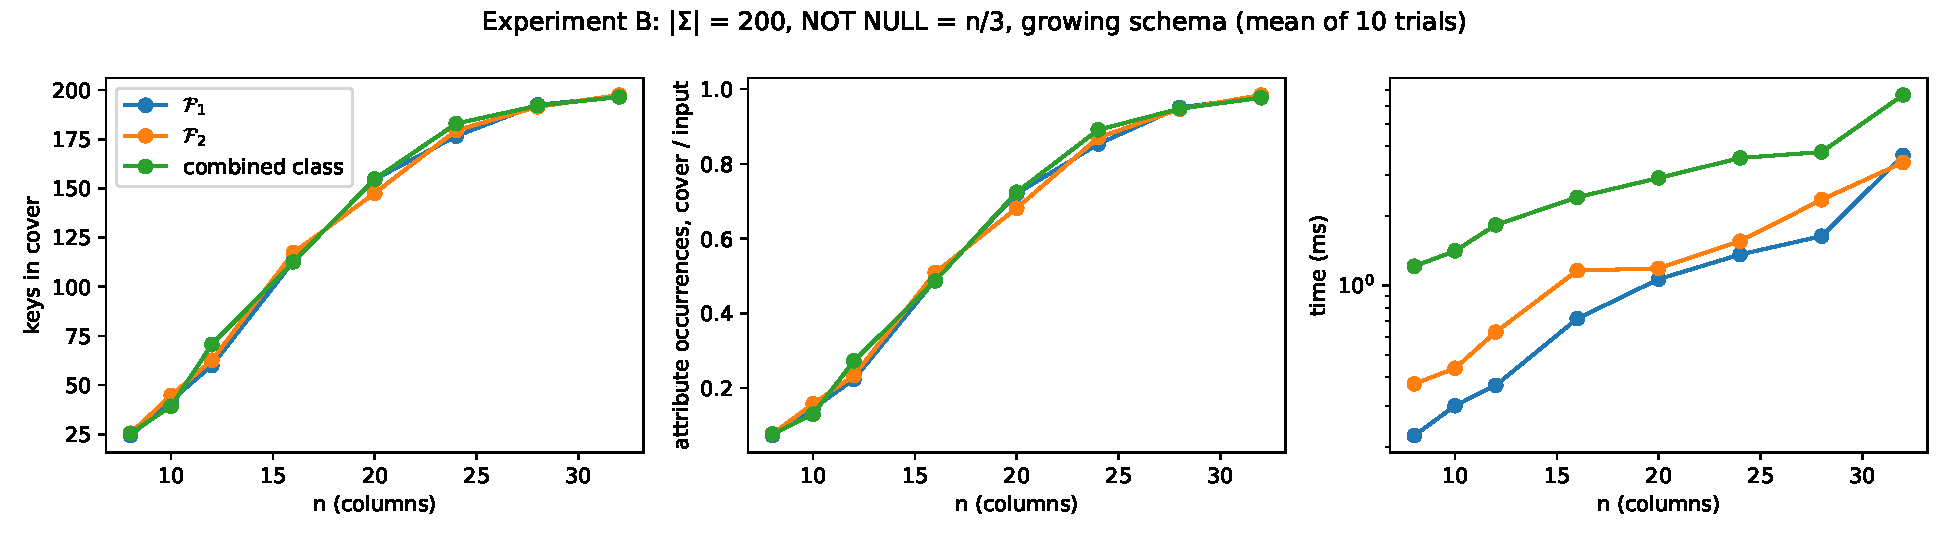
\includegraphics[width=0.9\textwidth]{figs/expB.pdf}
\caption{Experiment B: $|\Sig|=200$ random keys, \sql{NOT NULL} on $n/3$ columns,
schema size growing from 8 to 32 columns.}
\label{fig:expB}
\Description{}
\end{figure*}

\FloatBarrier
\subsection{Absolute times of Experiment D}\label{app:expD}

Figure~\ref{fig:expDboth} and Table~\ref{tab:expDratio} in
Section~\ref{sec:experiments} report Experiment D as speed-ups. This appendix gives
the absolute numbers behind them, per engine. Figure~\ref{fig:expD} and
Table~\ref{tab:expD} are the SQLite run (SQLite~3.45, in memory), with a fourth
panel showing the number of indexes created; Figure~\ref{fig:expDpg} and
Table~\ref{tab:expDpg} are the PostgreSQL~16 run on the same inputs, covers and
workloads. Both tables list, for each fragment and input size, the keys of input
and cover, the filtered indexes and trigger probes created, and the seconds for
1500 inserts, 600 updates and the integrity check, input / cover, as means over 5
runs. The number of indexes and probes is the same on both engines, since the
schemas are the same; only the times differ. Two differences between the engines
stand out. Absolute times on PostgreSQL are 10--50 times higher, as each statement
is a client--server round trip with its own savepoint rather than a call into an
in-process database. And the integrity check of the input is far slower on
PostgreSQL at large $|\Sig|$ (110--300\,s against 0.2--0.7\,s), because the planner
considers every one of the table's 400--600 partial indexes when it plans each
self-join, as discussed in Section~\ref{sec:experiments}; SQLite's planner does
not, so its check gains only 1.4--3.6 times from the cover.

\begin{figure*}[t]
\centering
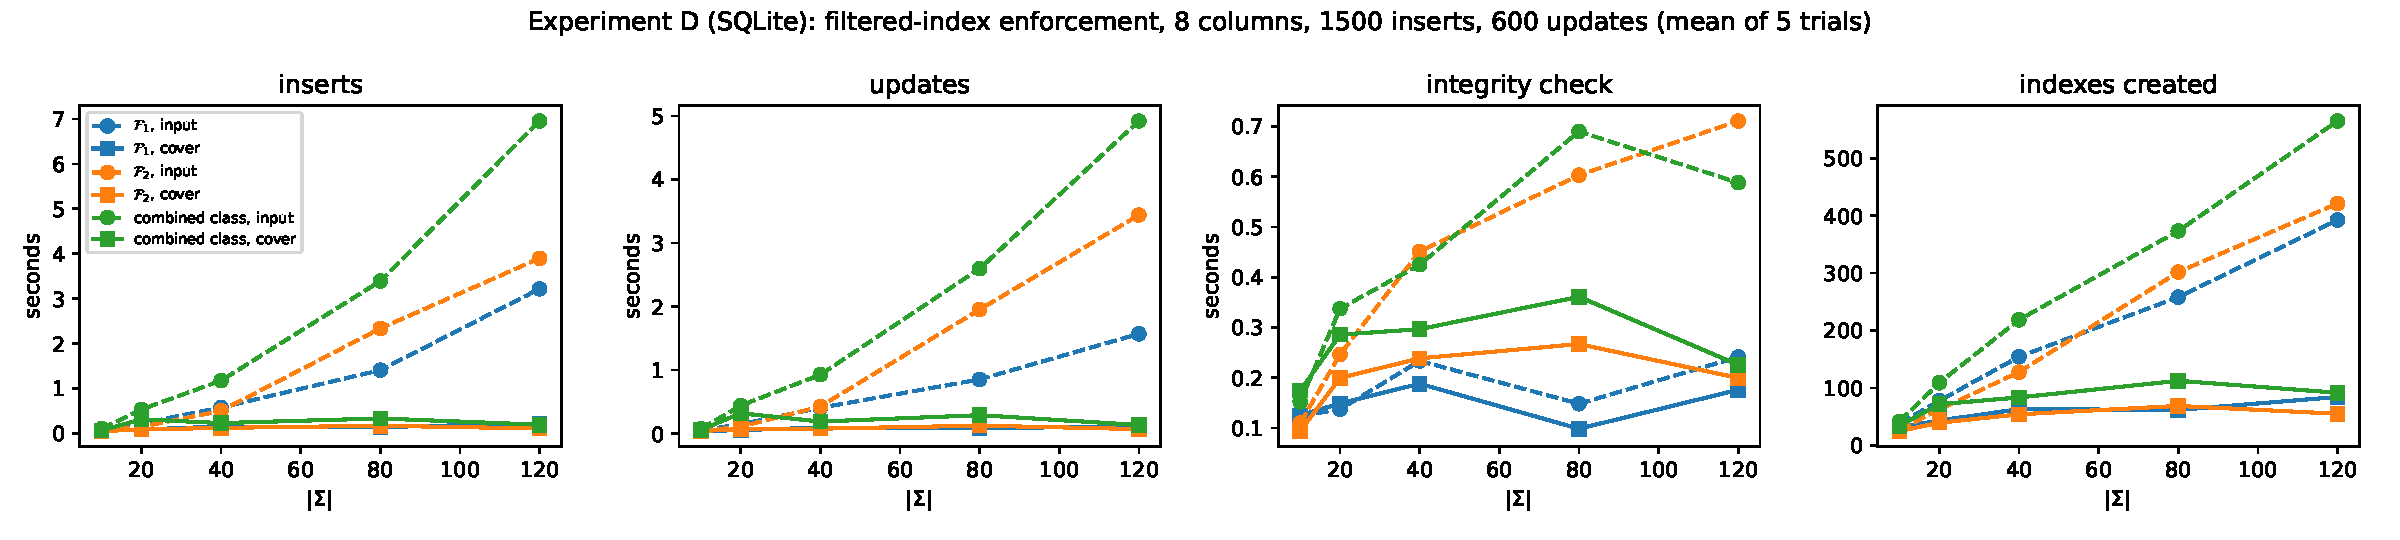
\includegraphics[width=0.9\textwidth]{figs/expD.pdf}
\caption{Experiment D: enforcing the input (dashed) and its cover (solid) with
filtered unique indexes and pattern-dispatched triggers on an 8-column table;
1500 inserts, 600 updates, a full integrity check, and the number of indexes
created.}
\label{fig:expD}
\Description{}
\end{figure*}
\begin{figure*}[t]
\centering
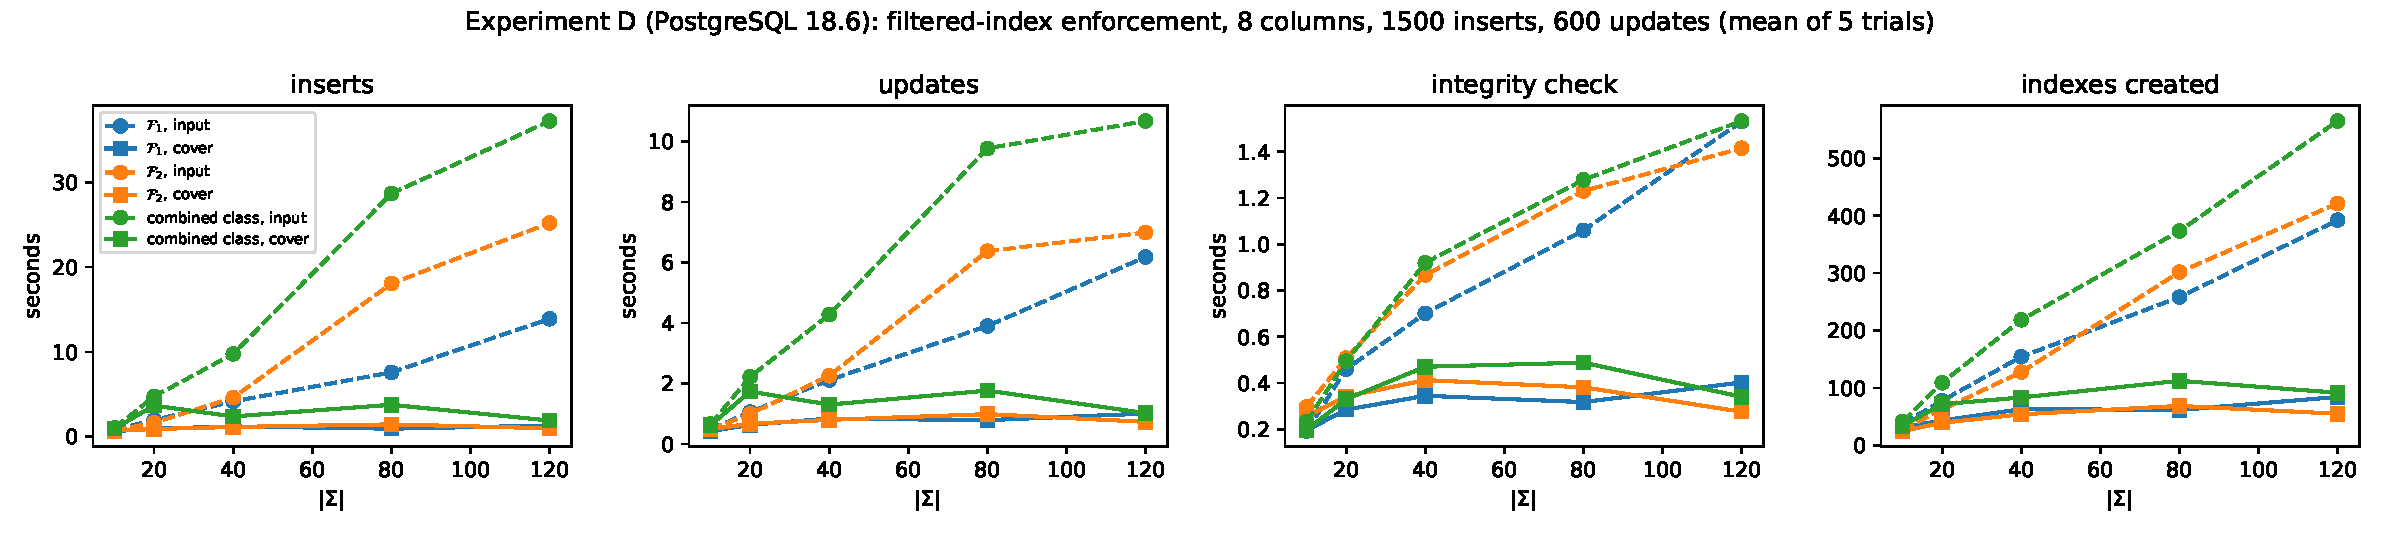
\includegraphics[width=0.9\textwidth]{figs/expD_pg.pdf}
\caption{Experiment D on PostgreSQL~16: enforcing the input (dashed) and its
cover (solid) with native \sql{NULLS NOT DISTINCT} and partial unique indexes and
PL/pgSQL pattern-dispatched triggers; same workload as Figure~\ref{fig:expD}.}
\label{fig:expDpg}
\Description{}
\end{figure*}

\begin{table*}[t]
\centering
\caption{Experiment D, means over 5 runs: keys of input and cover, filtered
indexes and trigger probes created, and seconds for 1500 inserts, 600 updates and
the integrity check, input / cover}
\label{tab:expD}
\small
\adjustbox{max width=\textwidth}{\begin{tabular}{l r r rr rr rr rr rr}
\toprule
Fragment & $|\Sig|$ & $|\Gamma|$ & \multicolumn{2}{c}{indexes} & \multicolumn{2}{c}{probes} & \multicolumn{2}{c}{inserts} & \multicolumn{2}{c}{updates} & \multicolumn{2}{c}{check} \\
\midrule
$\mathcal F_1$ & 10 & 7.4 & 38 & 31 & 64 & 54 & 0.09 & 0.07 & 0.05 & 0.04 & 0.12 & 0.12 \\
& 40 & 16.8 & 154 & 63 & 260 & 110 & 0.58 & 0.15 & 0.41 & 0.09 & 0.23 & 0.19 \\
& 120 & 27.0 & 392 & 84 & 618 & 140 & 3.22 & 0.22 & 1.57 & 0.12 & 0.24 & 0.18 \\
$\mathcal F_2$ & 10 & 8.0 & 27 & 25 & 40 & 38 & 0.06 & 0.05 & 0.04 & 0.04 & 0.11 & 0.09 \\
& 40 & 18.4 & 128 & 54 & 200 & 86 & 0.50 & 0.12 & 0.43 & 0.08 & 0.45 & 0.24 \\
& 120 & 19.8 & 421 & 55 & 685 & 94 & 3.90 & 0.11 & 3.44 & 0.07 & 0.71 & 0.20 \\
combined & 10 & 7.2 & 42 & 34 & 73 & 62 & 0.11 & 0.07 & 0.08 & 0.06 & 0.15 & 0.17 \\
& 40 & 17.4 & 219 & 83 & 402 & 154 & 1.18 & 0.23 & 0.93 & 0.19 & 0.42 & 0.30 \\
& 120 & 26.6 & 565 & 92 & 1009 & 164 & 6.95 & 0.19 & 4.92 & 0.14 & 0.59 & 0.23 \\
\bottomrule
\end{tabular}}
\end{table*}
\begin{table*}[t]
\centering
\caption{Experiment D on PostgreSQL~16, means over 5 runs, in the layout of
Table~\ref{tab:expD}: seconds for 1500 inserts, 600 updates and the integrity
check, input / cover}
\label{tab:expDpg}
\small
\adjustbox{max width=\textwidth}{\begin{tabular}{l r r rr rr rr rr rr}
\toprule
Fragment & $|\Sig|$ & $|\Gamma|$ & \multicolumn{2}{c}{indexes} & \multicolumn{2}{c}{probes} & \multicolumn{2}{c}{inserts} & \multicolumn{2}{c}{updates} & \multicolumn{2}{c}{check} \\
\midrule
$\mathcal F_1$ & 10 & 7.4 & 38 & 31 & 64 & 54 & 2.02 & 1.86 & 1.27 & 1.14 & 1.39 & 0.41 \\
 & 40 & 16.8 & 154 & 63 & 260 & 110 & 13.30 & 3.26 & 6.92 & 2.40 & 3.25 & 0.89 \\
 & 120 & 27.0 & 392 & 84 & 618 & 140 & 49.52 & 3.72 & 23.64 & 3.37 & 110.07 & 1.31 \\
$\mathcal F_2$ & 10 & 8.0 & 27 & 25 & 40 & 38 & 1.78 & 1.68 & 1.32 & 1.14 & 0.69 & 0.54 \\
 & 40 & 18.4 & 128 & 54 & 200 & 86 & 14.68 & 3.14 & 7.39 & 2.30 & 3.23 & 0.95 \\
 & 120 & 19.8 & 421 & 55 & 685 & 94 & 76.69 & 2.42 & 22.93 & 2.32 & 120.95 & 0.75 \\
combined & 10 & 7.2 & 42 & 34 & 73 & 62 & 2.74 & 2.68 & 1.76 & 1.62 & 0.62 & 0.48 \\
 & 40 & 17.4 & 219 & 83 & 402 & 154 & 30.69 & 7.31 & 13.59 & 4.13 & 5.32 & 1.24 \\
 & 120 & 26.6 & 565 & 92 & 1009 & 164 & 127.65 & 5.74 & 37.81 & 3.57 & 156.32 & 1.11 \\
\bottomrule
\end{tabular}}
\end{table*}
\FloatBarrier
\section{Logs and Reproducibility}\label{app:repro}

All artifacts---code, data, raw results and the build of both versions of this
paper---are available at \url{https://github.com/lshelloworld/one-cover-artifacts}.
Every generated input and its cover are written to \texttt{covers\_log.jsonl}
(560 records: fragment, $n$, $k$, the \sql{NOT NULL} set, the keys of input and
cover in the notation of this paper, their counts and attribute occurrences, and
the time) and \texttt{db2\_log.jsonl} (75 records, adding the numbers of indexes
and probes, accepted inserts and updates, and the three timings for input and
cover; \texttt{db\_log.jsonl} holds the naive-trigger run, and
\texttt{db2\_pg\_log.jsonl} the PostgreSQL run with the same fields plus the
index-creation time and a flag recording that the accepted statements agree
with the SQLite run). The scripts
\texttt{exp\_covers.py}, \texttt{exp\_db2.py} and \texttt{exp\_db.py} regenerate
all figures from fixed random seeds, and \texttt{experiments/pg/} holds the
generated PostgreSQL schemas (input and cover for each fragment and input size).
\texttt{exp\_db2\_pg.py} replays Experiment~D against a PostgreSQL server
through \texttt{psycopg2}, regenerating the inputs and workloads from the same
seed and asserting on every run that they match the logged ones; the SQLite runs
take under ten minutes, the PostgreSQL run about two and a half hours on one core.



\end{document}